%!TEX root = thesis.tex
\chapter{Homeotropic nematic bridges}

\section{Introduction}
The research presented so far has focused on nematic materials confined by toroidal surfaces.
Here we consider a NLC confined under homeotropic anchoring to a volume topologically like a sphere.
As established in Chapter~\ref{c:2}, the volume must contain a total hedgehog charge $|d| = 1$, with the hedgehog charge defined in Eq.~\ref{e:2-hedCharge}.
Using a single defect, this condition can be is satisfied by $d=-1$ hyperbolic point defects or hyperbolic ring defects, shown schematically from the side and top in Figure~\ref{f:2-3DMeas}(B,D), and also by $d=+1$ radial point defects or radial ring defects, shown schematically from the side and top in Figure~\ref{f:2-3DMeas}(A,C).
The myriad of possible defect configurations satisfying the topological constraints gives the system a richness that has been well-explored for the spherical case, where the confinement can only be modified through changing the sphere radius~\cite{RN150,RN277,RN278,RN275,RN276}.
However, the role of shape when confining NLC in geometries with more than one characteristic lengthscale is not completely understood.

Consider the case of a cylindrical geometry of aspect ratio $\Gamma = 2 R/H$, where $R$ is the radius of the cylinder and $H$ is its height.
With this notation, the classic case of a cylindrical capillary corresponds to $\Gamma \ll 1$. The $\Gamma \gg 1$ situation corresponds to confinement between narrowly separated plates.
When $\Gamma \sim \mathcal{O}\left( 1 \right)$, the equilibrium defect configuration undergoes a transition from a ring defect, found when $\Gamma \gg 1$, to a point defect, seen when $\Gamma \ll 1$.
Prior experimental work on the defect structure in liquid crystal bridges focused on the transition between the ring and the point defect as a function of $\Gamma$~\cite{RN139,RN147}.
However, we note that Refs.~\cite{RN139,RN147} only observed the bridge structures from above and thus were unable to determine how the bridge shape affects the defect transition.
In addition, since the radial and hyperbolic defects appear the same when viewed from above, as seen in the lower row in Figure~\ref{f:2-3DMeas}(A,B) and Figure~\ref{f:2-3DMeas}(C,D) for ring defects and point defects, respectively, Refs.~\cite{RN139,RN147} could not say whether the defects were radial or hyperbolic.
Prior theoretical work used computational modeling to explore the defect configuration within a cylindrical bridge as a function of $\Gamma$ and $K_{11}/K_{33}$~\cite{RN138,RN144}.
For 5CB, which has $K_{11}/K_{33} = 0.74$, they predicted that the bridge should transition between a radial ring defect [see Figure~\ref{f:2-3DMeas}(C)] and a hyperbolic point defect [see Figure~\ref{f:2-3DMeas}(B)].
However, as with the experimental work~\cite{RN139,RN147}, Refs.~~\cite{RN138,RN144} also do not investigate the role of the bridge shape.
Thus, the role of shape in setting the defect structure (ring or point) and type (hyperbolic and radial) remains an open question.

In this Chapter, we address this open question and perform experiments pertaining to a confined NLC within a capillary bridge sandwiched between two parallel plates of adjustable separation and hence of varying $\Gamma$.
By observing our experimental bridges from both the top and the side and comparing our observations with computations performed by our collaborators Shengnan Huang and Paul Goldbart, we find that the shape of the free surface controls whether the defect is radial or hyperbolic: waist-like bridges contain hyperbolic defects, and barrel-like bridges contain radial defects.
To accomplish this, we develop polarized epifluorescent microscopy (PFM), an imaging technique allowing us to distinguish radial and hyperbolic defect structures in scenarios where common OPM techniques fail.
In addition, we find good agreement between experiment and theory for the critical aspect ratio, $\Gamma_c$, at which the defect in the bridge undergoes a transition between a ring defect and a point defect.
Finally, we see that this transition is hysteretic, due to the metastability of the point defect.
Our results illustrate how shape and the nematic elasticity dictate defect structure in confined homeotropic nematics.




\section{Making capillary bridges}
To make a capillary bridge, we confine 5CB between two parallel glass microscope slides.
Prior to use, the slides were dip-coated with $0.1\%$ w/w lecithin in hexane and left to dry to enforce homeotropic anchoring~\cite{RN140}.
We set up an experiment to view a bridge from the top by first placing both microscope slides stacked on top of each other on the microscope stage.
We then epoxy the top plate to a rod affixed to a micromanipulator such that we can adjust the distance between the slides.
Note that this simple protocol ensures that the two microscope slides are parallel to each other and to the microscope stage.
After the epoxy hardens, we raise the top slide and use a glass capillary to place a $\sim$nL-volume drop of 5CB onto the bottom plate.
We then bring the top plate down until it makes contact with the sessile droplet and forms a capillary bridge.
The final experimental setup is depicted schematically in Figure~\ref{f:5-BuildSchemaic}(A).
\begin{figure}
  \centering
  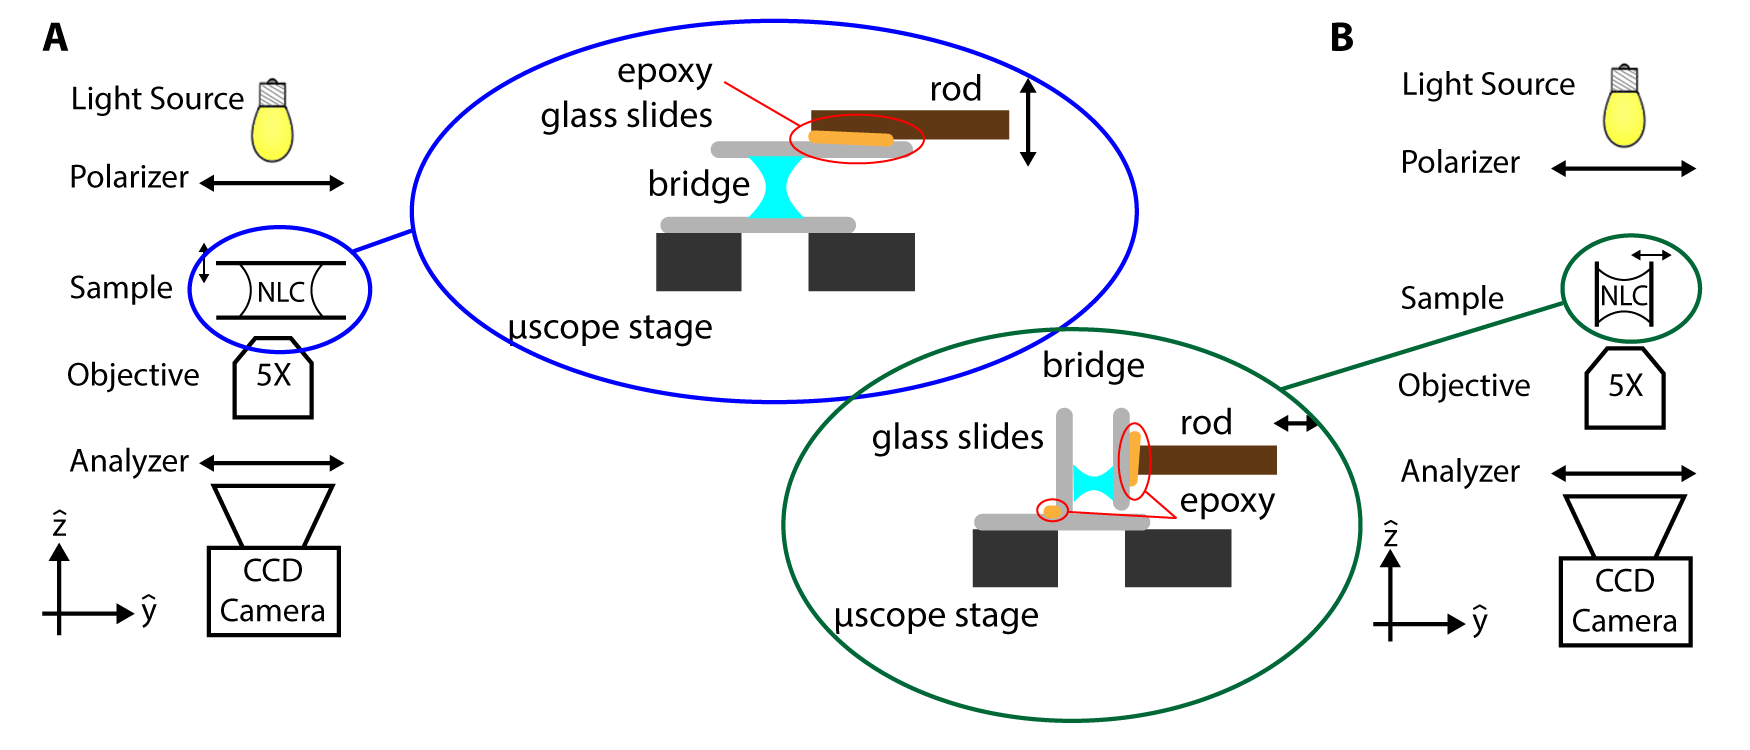
\includegraphics{figures/C5/Ch5-Figs_BuildSchematic.png}
  \caption{Experimental set-up.
  (A,B) Schematic from the side of the setup to view a bridge from the (A) top and (B) side.
  The zoomed-in portion of (A,B) highlights the setup to make and manipulate the bridge on the microscope stage.}\label{f:5-BuildSchemaic}
\end{figure}

To set up an experiment to view a bridge from the side, we place an uncoated glass slide on the microscope stage to act as a base, and then place a lecithin-coated glass slide vertically on the base and use a pair of blocks to hold it in place.
We then epoxy the lecithin-coated slide to the base, applying epoxy to only one side of the joint between the base and the lecithin-coated slide.
Once the epoxy has hardened, we remove the blocks and place the second lecithin-coated glass slide vertically on the base and against the previously-epoxied glass slide.
We then use the rod attached to the micromanipulator to hold the two vertical slides together while we epoxy the second lecithin-coated glass slide to the rod.
This protocol ensures that the two lecithin-coated glass slides are parallel to each other and perpendicular to the base.
After the epoxy hardens, we use the mircomanipulator to move the adjustable plate as far as possible from the fixed plate and place a $\sim$nl-volume drop of 5CB onto the fixed vertical plate as close to the base as we can.
Finally, we bring the adjustable plate closer to the fixed plate until it makes contact with the sessile drop and forms a capillary bridge.
The final experimental setup for a side view is depicted schematically in Figure~\ref{f:5-BuildSchemaic}(B).

As described, this procedure will yield a capillary bridge where the free-surface is in contact with air.
To make a capillary bridge with the free surface in contact with water, we first make a bridge as described above and then pipette a drop of water near the edge of the parallel plates and let capillary action fill the gap between the plates.
The water contains 8 mM SDS to enforce homeotropic anchoring.




\section{Shape of capillary bridges}
We begin by viewing the bridges from the side and characterizing their shapes.
Bridges with air as an outer medium have a waist-like shape with negative Gaussian curvature everywhere on the free surface, as shown by the bright-field image of an example bridge in Figure~\ref{f:5-ShapeContour}(A).
In contrast, as shown in the image of an example bridge in Figure~\ref{f:5-ShapeContour}(C), bridges with water and SDS as the outer medium have a barrel-like shape with positive Gaussian curvature everywhere on the free surface.
\begin{figure}
  \centering
  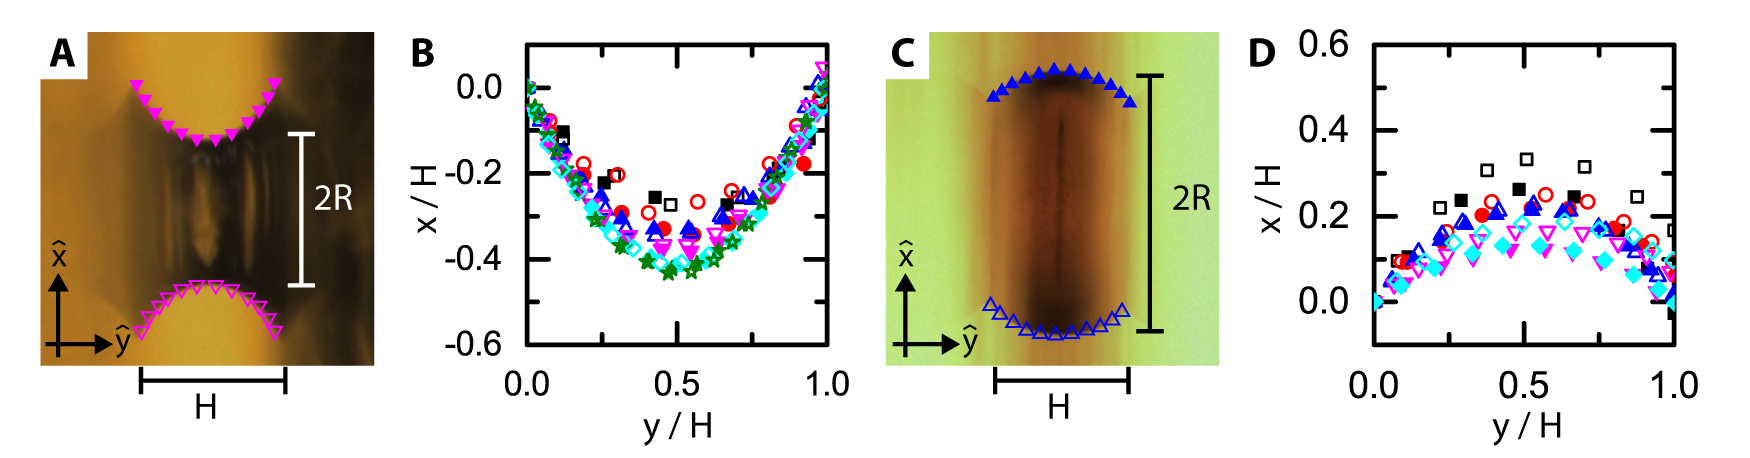
\includegraphics{figures/C5/Ch5-Figs_ShapeContour.png}
  \caption{Measuring the shape of a bridge.
  (A,C), Bright-field images from the side of a (A) waist-shaped and a (C) barrel-shaped bridge, with the effective radius $R$ and height $H$ of each bridge defined in the image.
  The waist in (A) has $R = 180$ $\upmu$m and $H = 170$ $\upmu$m, and the barrel in (C) has $R = 280$ $\upmu$m and $H = 300$ $\upmu$m.
  (B,D), Contours of the bridge shown in (A,C), respectively, at different $\Gamma = 2R/H$, where the positions have been scaled by $H$ and the (open symbols) lower contours have been reflected and shifted to line up with the (filled symbols) upper contours.
  The contours in (B) have (${\blacksquare,\, \square}$) $\Gamma = 7.3$,
   (${\color{red} \bullet,\, \circ}$) $\Gamma = 4.6$,
   (${\color{blue} \blacktriangle,\, \vartriangle}$) $\Gamma = 2.0$,
   (${\color{magenta} \blacktriangledown,\, \triangledown}$) $\Gamma = 1.0$,
   (${\color{cyan} \blacklozenge,\, \lozenge}$) $\Gamma = 0.6$, and
   (${\color{olive} \star,\, \star}$) $\Gamma = 0.4$.
  The contours in (D) have (${\blacksquare,\, \square}$) $\Gamma = 4.5$,
  ${\color{red} \bullet,\, \circ}$) $\Gamma = 3.9$,
  (${\color{blue} \blacktriangle,\, \vartriangle}$) $\Gamma = 1.9$,
  (${\color{magenta} \blacktriangledown,\, \triangledown}$) $\Gamma = 1.5$, and
  (${\color{cyan} \blacklozenge,\, \lozenge}$) $\Gamma = 1.3$.}\label{f:5-ShapeContour}
\end{figure}

\subsection{Measuring the shape}
As demonstrated on the example bridges in Figure~\ref{f:5-ShapeContour}(A,C), we record both the upper [closed symbols] and lower contours [open symbols] giving the shape of the bridge as a function of $\Gamma$, where we calculate an effective aspect ratio by taking $R$ as the radius of the circular cross-section of the bridge midway between the two confining plates and taking $H$ as the distance between the plates [see Figure~\ref{f:5-ShapeContour}(A,C)].
We then plot the contours normalized by the bridge height, with the lower contours reflected about the vertical axis, and all contours shifted so that their leftmost point corresponds to the origin, as shown in Figure~\ref{f:5-ShapeContour}(B,D) for the bridges in Figure~\ref{f:5-ShapeContour}(A,C), respectively.
For both the barrels and the waists, the respective contours all approximately have the same shape regardless of $\Gamma$ or experiment.


\subsection{Constant mean curvature surfaces}
To address the origin of the shape, we consider the relevant forces: the gravitational force $|\mathbf{F}_g| \sim \rho g R^2 H$; the surface tension force $|\mathbf{F}_{\gamma}| \sim \gamma H$; and the nematic elasticity force $|\mathbf{F}_K| \sim K$.
The surface tension, density, and Frank elastic constant of 5CB are equal, respectively, to $\gamma \approx 30$ mN/m, $\rho \approx 1$ g/mL, and $K \approx 10^{-11}$ N.
We compare these forces via two dimensionless groups: the Bond number $\rm{Bo} = \dfrac{|\mathbf{F}_g|}{|\mathbf{F}_{\gamma}|} = \dfrac{\rho g R^2}{\gamma} \sim  \mathcal{O}\left (10^{-2} \right)$, and the elasticity group,
 $\dfrac{|\mathbf{F}_{\gamma}|}{|\mathbf{F}_K|} =  \dfrac{\gamma H}{K} \sim \mathcal{O}\left (10^{5} \right )$, where we have taken $H = R = 100$ $\mu$m as representative values.
As $|\mathbf{F}_{\gamma}|$ is the dominant force, the mean curvature of the free surface of the bridge must be constant; otherwise, according to Eq.~\ref{e:3-LapPres}, there would be pressure gradients inside the bridge resulting in internal flow~\cite{RN178}.
Thus, the surface must satisfy:
\begin{equation}
  \Delta P = 2\gamma (-M) = -\gamma(\kappa_1 + \kappa_2) = \textrm{cons't},\label{e:5-ConsMeanCurv}
\end{equation}
where $\Delta P$ is the Laplace pressure, $M = {\rm tr}\{ \mathbf{L} \}/2 = (\kappa_1 + \kappa_2)/2$ is the mean curvature of the surface, and $\gamma$ is the surface tension.
In addition, note that our capillary bridges are surfaces of revolution, where a planar curve is rotated about an axis to form a surface.

We can gain further insight into the shape of our bridges by writing Eq.~\ref{e:5-ConsMeanCurv} in terms of a contour of a surface of revolution.
We can characterize such a contour in cylindrical coordinates $\{r,\varphi, z\}$, as schematically illustrated by the blue line in Figure~\ref{f:5-ShapeEnvelope}(A), with the arclength parameter, $s$, and the angle between the $r$-axis and the tangent to the contour at $s$,  $\theta$, the elevation angle.
The elevation angle naturally provides the contact angle for the surface, $\theta_0 = \theta(s=0)$, with $\theta_0$ the contact angle [blue circle, Figure~\ref{f:5-ShapeEnvelope}(A)].

For a surface of revolution in cylindrical coordinates, the principle curvatures are given by~\cite{RN35}:
\begin{equation}
  \kappa_1 = \frac{z''(r)}{(1+z'(r))^{3/2}}, \quad \kappa_2 = -\frac{z'(r)}{r\sqrt{1 + z'(r)^2}}.\label{e:5-SoRcurvatures}
\end{equation}
We can easily write ${\rm d}r/{\rm d}s$ and ${\rm d}z/{\rm d}s$ in terms of the elevation angle, ${\rm d}r/{\rm d}s = \cos \theta$ and ${\rm d}z/{\rm d}s = \sin \theta$, implying that $z'(r) = \tan \theta$.
% We can check these expressions using the relation ${\rm d}s^2 = {\rm d}r^2 + {\rm d}z^2$,
% \begin{align}
%   {\rm d}s^2 &= {\rm d}r^2 + {\rm d}z^2, \\
%   \frac{{\rm d}s^2}{{\rm d}r^2} &= 1 + z'(r)^2, \\
%   z'(r)^2 &= \sec^2 \theta - 1, \\
%   z'(r) &= \tan \theta, \label{e:4-zprime}
% \end{align}
% as desired.
Now, substituting this into Eqs.~\ref{e:5-SoRcurvatures}, we can write our principle curvatures in terms of $\theta$:
\begin{align}
  \kappa_1 = \frac{1}{R_1} &= \frac{\frac{\rm d}{{\rm d}r} \tan \theta}{(1 + \tan ^2 \theta)^{(3/2)}}, \\
           &= \frac{\frac{{\rm d}\theta}{{\rm d}r} \frac{\rm d}{{\rm d}\theta} \tan \theta}{\sec^3 \theta}, \\
           &= \frac{{\rm d}\theta}{{\rm d}s} \frac{{\rm d}s}{{\rm d}r} \cos \theta, \\
           &= \frac{{\rm d}\theta}{{\rm d}s}.\label{e:5-kappa1} \\
  \kappa_2 = \frac{1}{R_2} & = -\frac{\tan\theta}{r \sqrt{1 + \tan^2\theta}} \\
           &= -\frac{\sin \theta}{r}.\label{e:5-kappa2}
\end{align}

From Eq.~\ref{e:5-kappa1}, we can write $ds = R_1 d\theta$, which makes sense considering that $\theta(s)$ is also the angle between $\hat{z}$ and the normal to the curve at $s$; the first principle curvature describes how the surface changes in the $rz$-plane.
Similarly, from Eq.~\ref{e:5-kappa2}, we can write $R_2 = r/\sin\theta$, showing that the second radius of curvature is the distance from the contour to the z-axis along the normal to the contour.
More importantly, this shows that $R_2$ always originates on the $z$-axis for a surface of revolution.
Finally, if our bridges truly are surfaces of revolution with constant mean curvature, then the contours in Figure~\ref{f:5-ShapeContour}(B,D) must satisfy:
\begin{align}
  \frac{\textrm{d}\theta}{\textrm{d}s} &= \frac{\sin \theta}{r} - \frac{\Delta P}{\gamma},\label{e:5-ShapeSolveA} \\
  \frac{{\rm d}r}{{\rm d}s} &= \cos \theta, \\
  \frac{{\rm d}{z}}{{\rm d}s} &= \sin \theta.\label{e:5-ShapeSolveC}
\end{align}

These three equations can be solved with three initial conditions where $s = 0$.
We control the height of the bridge in our experiments, determining $z(s = 0)$.
As mentioned earlier, the contact angle is the initial condition on $\theta$, $\theta_0 = \theta(s=0)$.
Finally, since the volume is fixed in our experiments, this determines the final condition $r(s=0)$.
However, since the contours in Figure~\ref{f:5-ShapeContour}(B,D) have all been scaled by $H$ as well as all been shifted to all begin at $(0,0)$, the actual values of $z(s = 0)$ and $r(s = 0)$ do not affect the shape.
Accordingly, the difference between the contours for a waist [Figure~\ref{f:5-ShapeContour}(B)] and the contours for a barrel [Figure~\ref{f:5-ShapeContour}(D)] can only come from $\theta_0$.
Thus, the contact angle between the lecithin-coated glass slide, the outer medium, and the 5CB determines the shape of our bridges~\cite{RN178}.
\begin{figure}
  \centering
  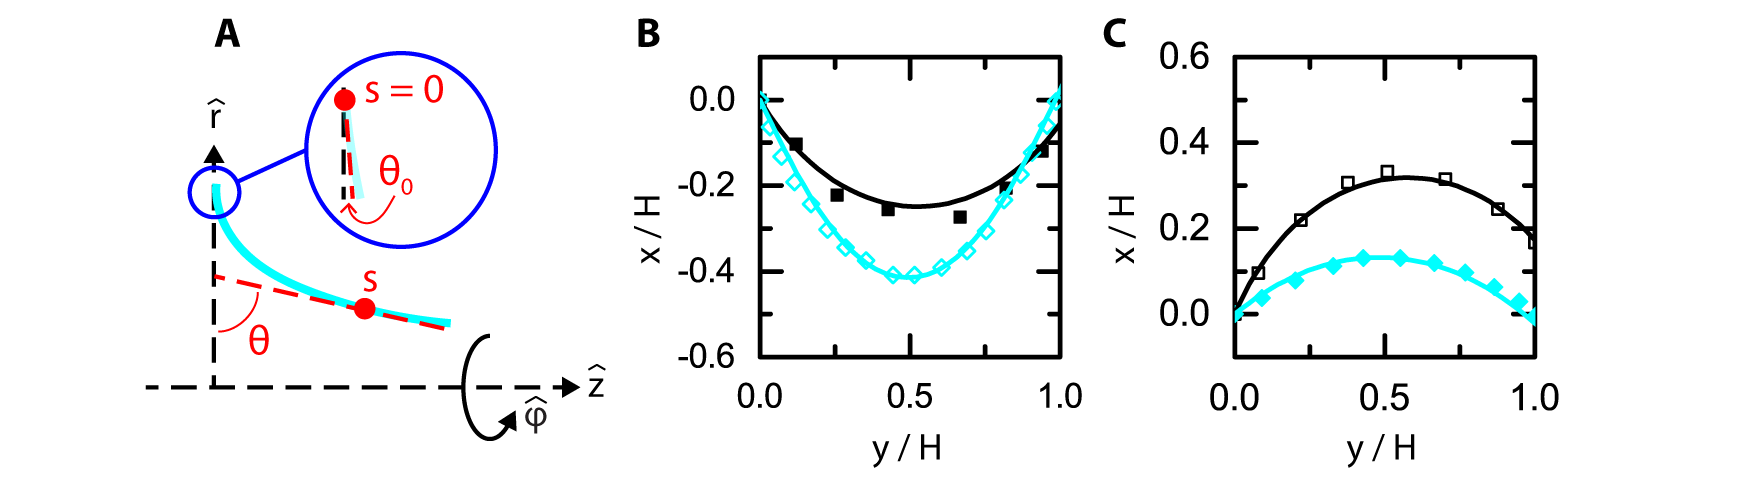
\includegraphics{figures/C5/Ch5-Figs_ShapeEnvelope.png}
  \caption{Constant mean curvature surfaces.
  (A), The elevation angle $\theta$ and arclength parameter $s$ defined for a surface of revolution in cylindrical coordinates, $\{r,\varphi, z\}$, with a contour of the surface displayed in cyan.
  $\theta$ is the angle between the tangent of the cyan curve at $s$ and $\hat{r}$.
  $\theta(s=0) = \theta_0$, the contact angle, as shown in the magnified section in the blue circle.
  (B,C), Numerically calculated contours for a constant mean curvature surface of revolution plotted on experimentally measured contours for a (B) waist and a (C) barrel.
  The numerical solutions have contact angles (B) (black line) $\theta_0^{waist} = 37^{\circ}$, (cyan line) $\theta_0^{waist} = 35^{\circ}$ and (C) (black line) $\theta_0^{barrel} = 149^{\circ}$, (cyan line) $\theta_0^{barrel} = 120^{\circ}$.
  The measured contours in (B,C) are reproduced from Figure~\ref{f:5-ShapeContour}(B,D), respectively, and form the envelope of the measured contours in Figure~\ref{f:5-ShapeContour}(B,D).}\label{f:5-ShapeEnvelope}
\end{figure}

To confirm this, we consider each bridge and numerically integrate Eqs.~\ref{e:5-ShapeSolveA}--\ref{e:5-ShapeSolveC} to produce constant-mean curvature contours that capture the observed contours in Figure~\ref{f:5-ShapeContour}.
We consider datasets in these figures representative of the spread observed, see Figure~\ref{f:5-ShapeEnvelope}(B,C).
To generate the numerical contours we start by making Eqs.~\ref{e:5-ShapeSolveA}--\ref{e:5-ShapeSolveC} dimensionless by dividing all lengths with $H$, such that $z(s = 0) = -1/2$ and $r(s = 0) = \Gamma/2$.
Note that since $\Gamma$ is measured in the middle of the two plates, $r(s = 0) = \Gamma/2$ is not accurate, but since the contours are shifted to all start at the same point, we emphasize again that $r(s = 0)$ doesn't affect the final shape.
We then numerically integrate Eqs.~\ref{e:5-ShapeSolveA}--\ref{e:5-ShapeSolveC} from $s = 0$ to $s = s_{lim}$, where $z(s = s_{lim}) = 1/2$, varying $\theta_0$ and $\Delta P$ until the numerical contours capture the experimental data, see Figure~\ref{f:5-ShapeEnvelope}(B,C).
For an ideal bridge where $r(s = 0) = r(s = s_{lim})$ and $\theta(s_{lim}) = \pi - \theta_0$ [blue contour, Figure~\ref{f:5-ShapeEnvelope}(B)], $\Delta P$ is not a free parameter but is determined by the constraints on $r(s = s_{lim})$ and $\theta(s_{lim})$.
However, the contact areas on the plates are not always equal in our experiments, making $r(s = 0) \neq r(s = s_{lim})$ [black contour, Figure~\ref{f:5-ShapeEnvelope}(C)].
Here, we vary $\Delta P$ for a given $\theta_0$ to best fit the data, changing $r(s = s_{lim})$ and $\theta(s_{lim})$.
We average the contact angles from the numerically-integrated contours for the waists and barrels to get $\theta^{waist}_0 = 36^{\circ} \pm 8^{\circ}$ and $\theta^{barrel}_0 = 127^{\circ} \pm 9^{\circ}$.
We compare the contact angles determined from our calculated contours with contact angles measured from sessile droplets with both air and water as the outer medium, finding $\theta_0^{air} = 37^{\circ} \pm 5^{\circ}$ and $\theta_0^{water} = 123^{\circ} \pm 5^{\circ}$.
This is in agreement with our data from the bridges, confirming that the contact angle is the main parameter determining the shape of our bridges.




\section{Defect structure transitions}
We view the bridge from the top to determine whether the defect is a ring or a point; examples of these situations are shown in the bright-field images of a waist-like bridge in Figure~\ref{f:5-ExpWaistTop}(A,C) and the corresponding crossed-polar images in  Figure~\ref{f:5-ExpWaistTop}(B,D).
\begin{figure}
  \centering
  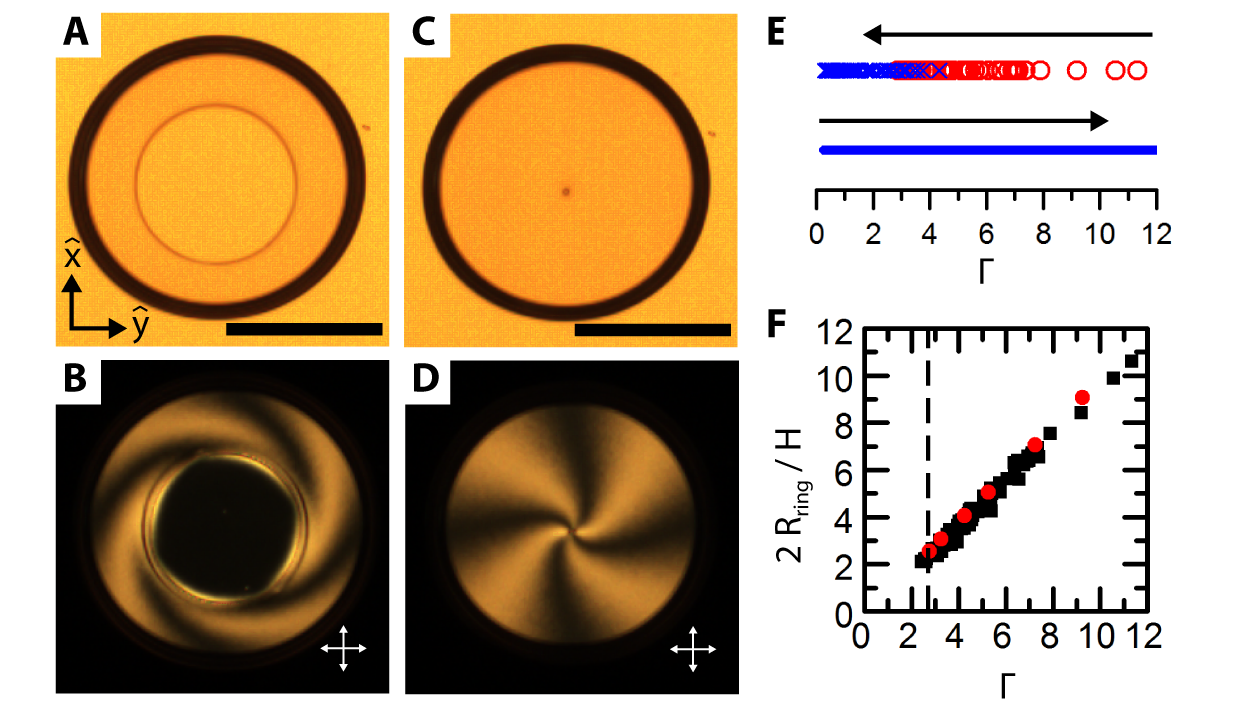
\includegraphics{figures/C5/Ch5-Figs_ExpWaistTop.png}
  \caption{Data for bright-field and optical-polarized microscopy of waist-shaped NLC bridges viewed from the top.
  (A) Example bright-field image of a waist-shaped bridge with a ring defect.
  (B) Crossed-polar image of the bridge in (A).
  (C) Example bright-field image of a waist-shaped bridge with a point defect. This is the same bridge as in (A), but with an increased distance between the plates.
  (D) Crossed-polar image of the bridge in (C).
  (E) Experimental phase diagram for the defect state, demonstrating hysteresis at the transition.
  The arrows indicate the directions in which $\Gamma$ is changed in the experiments.
  Starting at a large $\Gamma$ in the ring-defect state (${\color{red} \circ}$) and decreasing $\Gamma$ leads to a transition to a point defect (${\color{blue} \times}$) at a value of $\Gamma = 2.7 \pm 0.3$, which we obtain by averaging the result for all bridges.
  In contrast, when starting at small $\Gamma$ in a point-defect state and increasing $\Gamma$, the point-defect state persists; this is represented with a line.
  (F) The ring defect diameter in a waist-shaped bridge scaled by half the bridge height, plotted as a function of the bridge aspect ratio. A vanishing ring radius corresponds to a point defect.
  The ($\blacksquare$) are experimental measurements; the (${\color{red} \bullet}$) correspond to computations in a waist structure using the elastic constants for 5CB.\@
  Scale bars in (B,D): 250 $\upmu$m.}\label{f:5-ExpWaistTop}
\end{figure}

\subsection{Defect transitions in a waist}
We start at large $\Gamma$, where the equilibrium state has a ring defect, and determine the radius of the ring, $R_{ring}$, as we decrease $\Gamma$ by increasing $H$ in discrete steps.
At each $H$, we monitor the bridge over time to ensure that the defect state no longer changes and the system is in equilibrium.
In addition, as we decrease $\Gamma$ in each bridge, we also determine the effective aspect ratio for the defect transition, $\Gamma_c$.
Using results for 21 different bridges, we find an average $\Gamma_c = 2.7 \pm 0.3$, as shown in the upper contour in Figure~\ref{f:5-ExpWaistTop}(E), where we have plotted each observation of a stable ring defect with a (${\color{red} \circ}$) symbol and each observation of a stable point defect with a (${\color{blue} \times}$) symbol.
The ring diameter, scaled by the bridge height, varies linearly with $\Gamma$ for $\Gamma > \Gamma_c$, as indicated by the squares in Figure~\ref{f:5-ExpWaistTop}(F), where we have again plotted every measurement we have performed.
At $\Gamma_c$, the  ring becomes unstable, and collapses to a point defect, yielding the discontinuity in $R_{ring}$ shown with a dashed line in Figure~\ref{f:5-ExpWaistTop}(F), where the point defect is represented as having a vanishing $R_{ring}$.

However, when we start at $\Gamma < \Gamma_c$ in a point defect state and increase $\Gamma$, the point defect never transitions to a ring, as seen in the lower contour in Figure~\ref{f:5-ExpWaistTop}(E).
Interestingly, if for $\Gamma > \Gamma_c$, we melt the nematic phase in a bridge containing a point defect, we always recover a ring defect state when we let the bridge cool back to the nematic phase.
In contrast, when we do this for $\Gamma < \Gamma_c$, we still find a point defect when we let the bridge cool back to the nematic phase.
This suggests that the point defect is metastable for $\Gamma > \Gamma_c$.


\subsection{Defect transitions in a barrel}
% Since every barrel-shaped bridge we make initially starts as a waist, we need to make sure the defect state in the waist does not affect the final state in the barrel.
% Thus, we make our barrels both from waists with the 5CB in the nematic phase and from waists where the 5CB has been melted to the isotropic phase before adding the water and SDS mixture.
% For the barrels made with the 5CB in the isotropic phase, we also heat the water and SDS mixture before making the barrel so that the 5CB does not cool to the nematic phase before the barrel shape has been established.
As with the waist structures, we start with a large $\Gamma$ where the bridge contains a ring defect and decrease $\Gamma$ in discrete steps, measuring the ring radius at each step, as shown in the bright field images of a barrel for four values of $\Gamma$ in Figure~\ref{f:5-ExpBarrelTop}(A,C,E,G), with the associated crossed-polar images in Figure~\ref{f:5-ExpBarrelTop}(B,D,F,H).
However, over time the SDS forms micelles in the 5CB that self-assemble onto the ring defect and form visible structures [see Figure~\ref{f:5-ExpBarrelTop}(E,G)] in the NLC~\cite{RN279}.
In addition, note how the area inside the ring defect in the OPM images in in Figure~\ref{f:5-ExpBarrelTop}(B,D,F,H) becomes progressively brighter over time.
Since the SDS micelles themselves are not birefringent, this brightening implies that the micelles are affecting the director field inside the bridge.
Recall that the director field for a ring defect viewed from the top [see Figure~\ref{f:2-3DMeas}(C,D)] indicates that the area bounded by the ring should be dark when the polarizer and analyzer are crossed.
For a waist, where there is no SDS, this is always true [see Figure~\ref{f:5-ExpWaistTop}(B)].
In addition, we see that the self-assembled micelles can even stabilize non-circular ring shapes [see Figure~\ref{f:5-ExpBarrelTop}(G)] and off-center rings [see Figure~\ref{f:5-ExpBarrelRing}(B)], further indicating that the SDS can affect the director field in our bridges~\cite{RN279,RN280}.
\begin{figure}
  \centering
  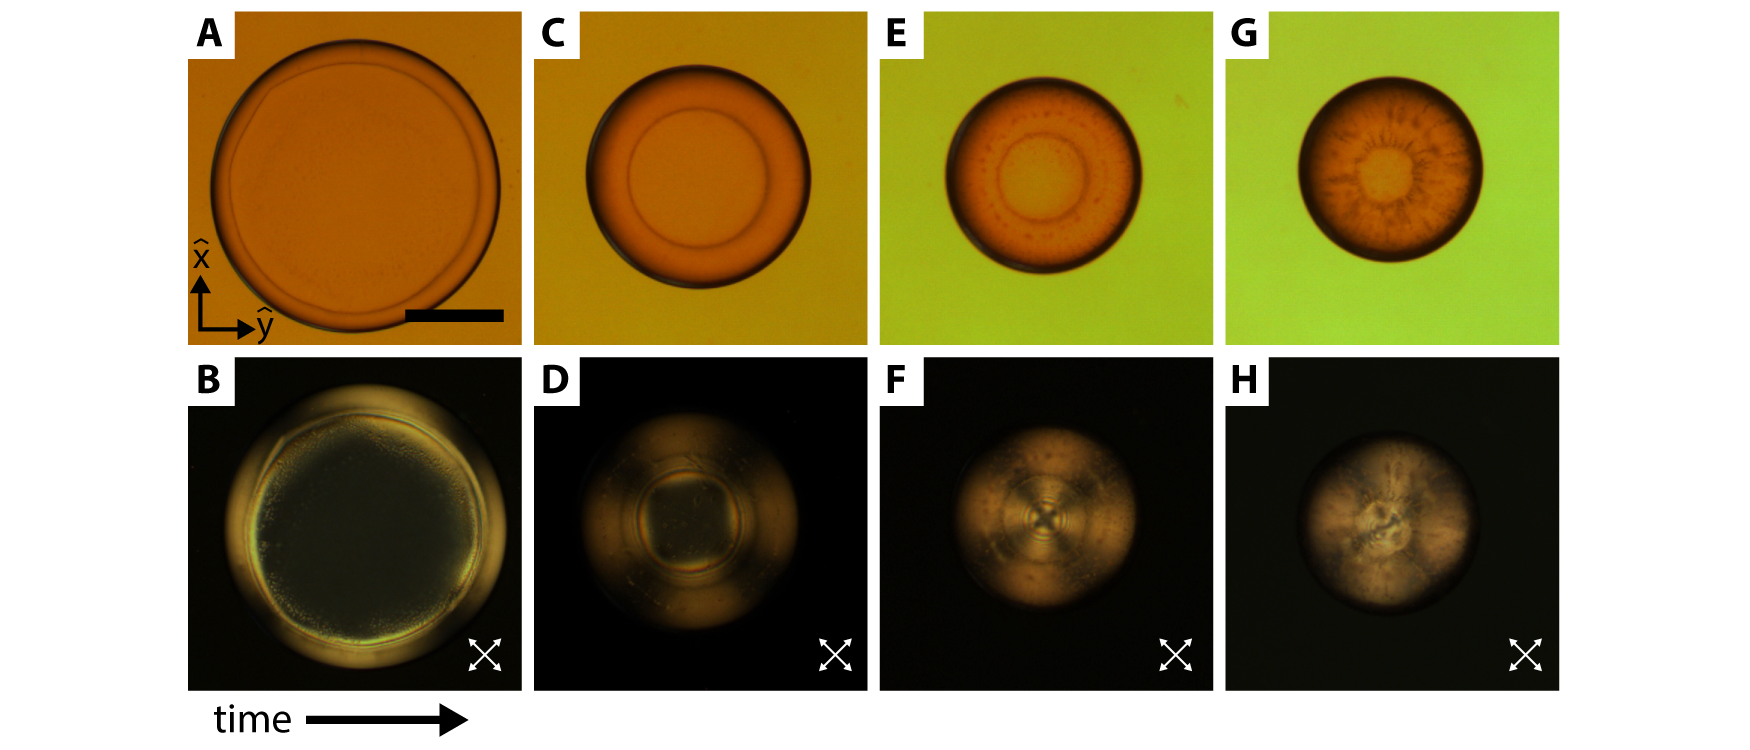
\includegraphics{figures/C5/Ch5-Figs_ExpBarrelTop.png}
  \caption{Bright-field and optical-polarized microscopy of barrel-shaped NLC bridges viewed from the top.
  (A,C,E,G), Bright-field images of a barrel-shaped bridge viewed from top with (A) $\Gamma = 5.0$, (C) $\Gamma = 2.6$, (E) $\Gamma = 1.4$, and (G) $\Gamma = 0.9$.
  Measurements were taken starting at (A) with $\Gamma = 5.0$ and decreasing $\Gamma$ in discrete steps.
  (B,D,F,H), Corresponding crossed-polar images of the bridges in (A,C,E,G), respectively.
  Note how the sodium dodecyl sulfate (SDS) used to enforce homeotropic anchoring in the barrels forms micelles and disrupts the director in the bridge over time, from the initial measurement in (A,B) to the final measurement pictured in (G,H).
  The scale bar in (A) is $250$ $\upmu$m.}\label{f:5-ExpBarrelTop}
\end{figure}

To minimize the effect of the SDS micelles, we restrict our measurements to ring defects that are circular and centered in the bridge.
We also make sure that the region within the ring in the crossed-polar images is dark, indicating that the SDS micelles have not yet significantly affected the NLC.
For example, we exclude the data in Figure~\ref{f:5-ExpBarrelTop}(E-H) and in Figure~\ref{f:5-ExpBarrelRing}(B,C).
We then plot the ring diameter scaled by the bridge height as a function of $\Gamma$ for each bridge, as seen in Figure~\ref{f:5-ExpBarrelRing}(A).
Here, the data are color coded by the measurement number for each bridge; the first measurement we make on a particular bridge is indicated by the (${\blacksquare,\, \square}$) symbols.
We then decrease $\Gamma$ and make the second measurement for that bridge, plotting the data with the (${\color{red} \blacksquare,\, \square}$) symbols.
Similarly, the third and fourth measurements on a bridge are indicated by the (${\color{blue} \blacksquare,\, \square}$) and (${\color{magenta} \blacksquare,\, \square}$) symbols, respectively.
The few magenta and blue points compared to the number of black and red points in Figure~\ref{f:5-ExpBarrelRing}(A) indicate that the effect of the micelles grows in time; we, in fact, rarely have good data to make a fourth measurement and we never have good enough data to make a fifth measurement for a given bridge.
Thus, even though we see that the scaled ring diameter varies linearly with $\Gamma$, [Figure~\ref{f:5-ExpBarrelRing}(A)], we cannot make a quantitative prediction about a ring-to-point defect transition in our barrel-shaped bridges.
This is true regardless of whether we make a barrel by adding the water + SDS to a waist with the 5CB in the nematic state [open squares, Figure~\ref{f:5-ExpBarrelRing}(A)] or with the 5CB in the isotropic state [closed squares, Figure~\ref{f:5-ExpBarrelRing}(A)].
In addition, note that the protocol used to make the barrel does not affect how the scaled ring diameter depends on $\Gamma$, indicating that the defect state in a barrel is not affected by the waist it was made from.

Even when we make barrels where the first measurement has low $\Gamma$, we do not see a clear collapse to a point defect; instead, we see a small ring defect with $0 < 2 R_{ring}/H < 0.3$, as pictured in Figure~\ref{f:5-ExpBarrelRing}(B,C) and Figure~\ref{f:5-ExpBarrelRing}(D,E) for barrels made with $\Gamma = 2.4$ and $\Gamma = 2.8$, respectively.
Since the ring in Figure~\ref{f:5-ExpBarrelRing}(B) is off-center, we exclude this data.
For the ring in Figure~\ref{f:5-ExpBarrelRing}(D), we measure $2 R_{ring}/H =0.1$, and plot the data in Figure~\ref{f:5-ExpBarrelRing}(A).
We made ten barrels with an initial $\Gamma < 5$, we excluded seven of the barrels due to SDS effects.
The remaining three barrels all have $0 < 2 R_{ring}/H < 0.3$, as plotted in Figure~\ref{f:5-ExpBarrelRing}(A).
\begin{figure}
  \centering
  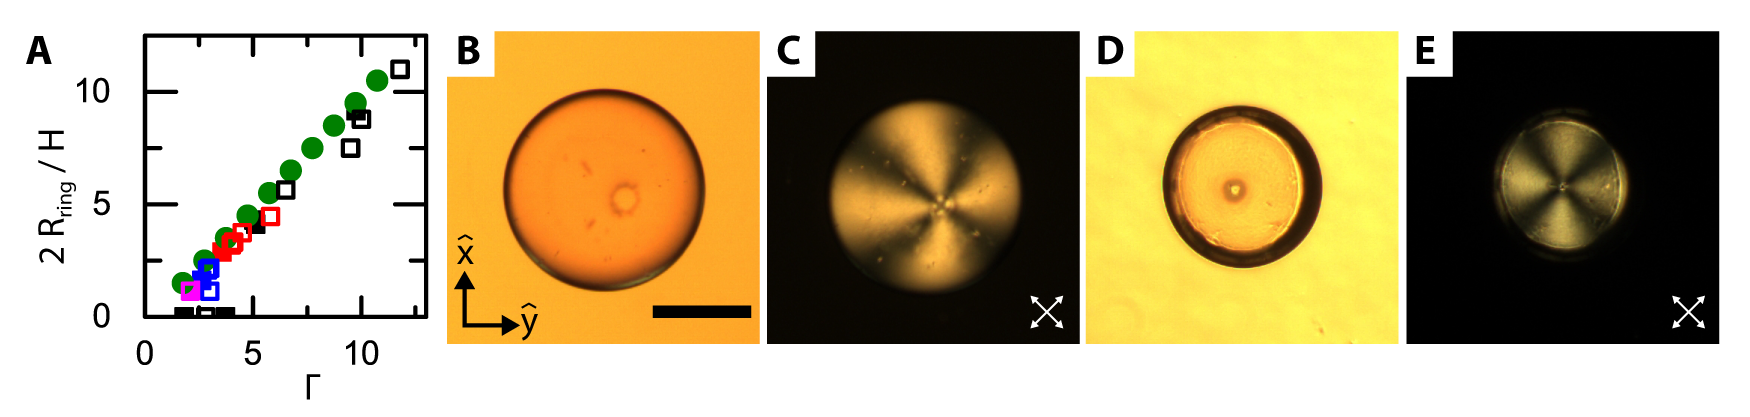
\includegraphics{figures/C5/Ch5-Figs_ExpBarrelRing.png}
  \caption{Ring defects in barrel-shaped NLC bridges viewed from the top.
  (A), The ring defect diameter in a barrel-shaped bridge scaled by height of the bridge divided by 2, plotted as a function of the bridge aspect ratio, $\Gamma$.
  The experimental points include barrels made with the 5CB in the [open squares] nematic phase and the 5CB in the [filled squares] isotropic phase.
  We label the experimental points with their measurement number, with (${\blacksquare,\, \square}$) corresponding to the first measurement, (${\color{red} \blacksquare,\, \square}$) the second measurement, (${\color{blue} \blacksquare,\, \square}$) the third measurement, and (${\color{magenta} \blacksquare,\, \square}$) the fourth measurement, where we start at a large $\Gamma$ and decrease $\Gamma$ with each subsequent measurement in a single barrel.
  The (${\color{olive} \bullet}$) correspond to computations in a barrel structure using the elastic constants for 5CB.\@
  (B--E), First measurement of a barrel with (B,C) $\Gamma = 2.4$ and (D,E) $\Gamma = 2.8$ made with the 5CB in the isotropic phase and viewed from the top just after the (B,D) bright field and (C,E) corresponding crossed-polar image indicate the director field has stopped changing.
  We exclude this bridge in (B,C) from the plot in (A) due to the presence of micelles; we cannot say if the micelles are preventing the ring from collapsing to a point defect of if the measured $2 R_{ring}/H = 0.2$ is the equilibrium state.
  The defect structure in (D,E) is a ring with $2 R_{ring}/H = 0.1$ and is plotted in (A) as such.
  The scale bar in (B) is 250 $\upmu$m.}\label{f:5-ExpBarrelRing}
\end{figure}




\section{Measuring defect conformation using fluorescence microscopy}
We return to viewing bridges from the side to determine if the defects are radial or hyperbolic.
We start by viewing the bridges with OPM and rotating the crossed polarizer and analyzer; the texture for a radial defect rotates in the same direction as the polarizer and analyzer, while the texture for a hyperbolic defect rotates with the opposite sense~\cite{RN177}.
However, due to the large curvature of the waist and barrel shapes, especially when $\Gamma$ is large, we cannot clearly distinguish the rotation of the texture.
This is demonstrated in Figure~\ref{f:5-PA_Rot} for a bridge with small $\Gamma$ [see Figure~\ref{f:5-PA_Rot}(A-C)] and a bridge with large $\Gamma$ [see Figure~\ref{f:5-PA_Rot}(D-F)].
Changing the polarizer and analyzer (P and A) orientations by 45$^{\circ}$ for the bridge with small $\Gamma$ [Figure~\ref{f:5-PA_Rot}(B,C)] produces a change in the texture, but it still does not clearly allow us to determine the brush rotation.
Rotating PA by 45$^{\circ}$ for the bridge with large $\Gamma$ [Figure~\ref{f:5-PA_Rot}(E,F)] produces an even smaller change in the texture.
As an alternative approach, we develop and use polarized epifluorescent microscopy (PFM) to see whether the defect is radial or hyperbolic.
\begin{figure}
  \centering
  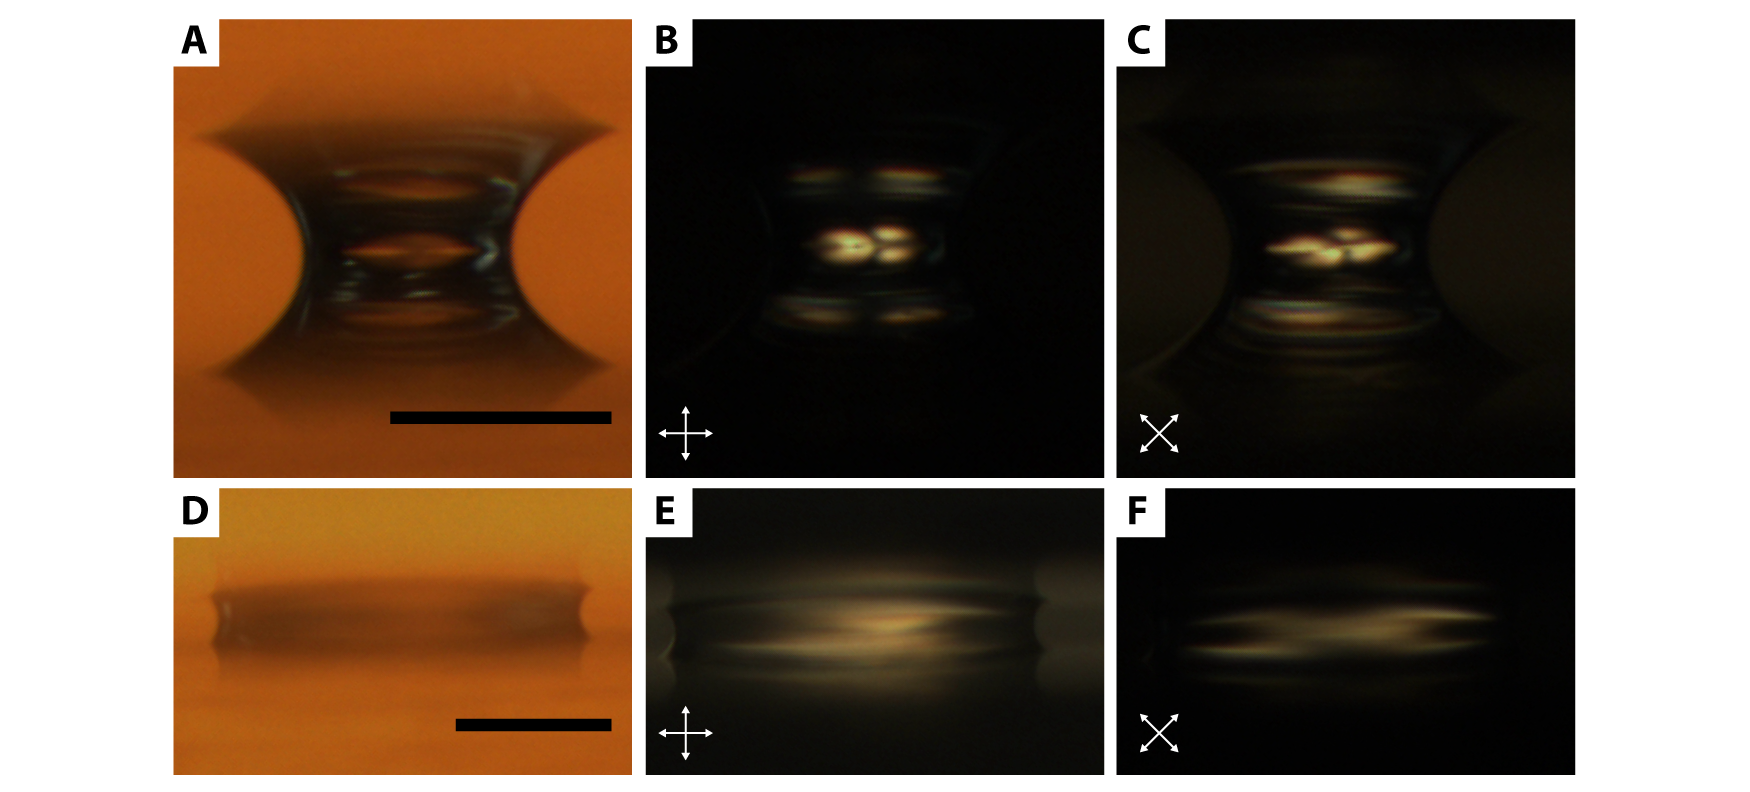
\includegraphics{figures/C5/Ch5-Figs_PA_Rot.png}
  \caption{Rotating the polarizer and analyzer for a waist-shaped bridge viewed with optical-polarized microscopy from the side.
  (A-C), A waist-shaped bridge with $\Gamma = 1.2$ viewed from the side under (A) bright field and (B,C) with crossed polarizer and analyzer (PA), where the PA orientations are specified in each image.
  (D-F), A waist-shaped bridge with $\Gamma = 6.6$ viewed from the side under (D) bright field and (E,F) with crossed PA, where the PA orientations are specified in each image.
  The scale bars in (A,D) are 250 $\upmu$m.}\label{f:5-PA_Rot}
\end{figure}

\subsection{Theoretical overview of polarized epifluorescent microscopy}
As mentioned earlier, fluorescence is an inelastic process where a material absorbs and then re-emits light.
The realization that this process consists of both absorption and emission of light is attributed to Stokes, as is the name ``fluorescence'' itself.~\cite{RN286,RN287}.
However, the understanding that fluorescent emission could be polarized came from Weigert's work with small fluorescent molecules, or fluorophores~\cite{RN285}.
Individual fluorophores absorb and emit light like dipoles, with the absorption/excitation dipole and the emission dipole not necessarily parallel to each other~\cite{RN282}.
Consequently, while an isotropic distribution of fluorophores will absorb and emit light isotropically, individual fluorophores are sensitive to the polarization of the excitation light and emit linearly polarized light along the emission dipole~\cite{RN282}.

Polarized fluorescence has proven to be an incredibly effective tool in diagnostic imaging and the medical community; for example, it is commonly used used to measure molecular or cellular mobility~\cite{RN282,RN284}.
Recently, the liquid crystal community has developed a renewed interest in polarized fluorescence, with techniques like Polarized Epifluorescent Confocal Microscopy (PCFM), enabling 3D resolution of a liquid-crystalline director~\cite{RN148,RN174}.
Here, we take inspiration from PCFM and develop Polarized Epifluorescent Microscopy (PFM), its wide-field cousin.
At its core, PFM relies on anisotropic fluorophores whose emission axis is aligned along the long axis of the fluorophore.
By introducing fluorophores in a NLC at low concentrations, the long axis of the fluorophores aligns along the nematic director without affecting the director configuration~\cite{RN148,RN174}.
Thus, the fluorescent emission of the mixed fluorophore and NLC system will be linearly polarized along the director.
If we excite the sample with unpolarized light and place an analyzer in the emitted light path, as depicted schematically in Figure~\ref{f:5-PFM_FlatCell}(A) then the emitted intensity from each point in the sample will be $\propto \cos^2{(\Phi_A-\delta)}$, where $\Phi_A$ is the orientation of the analyzer and $\delta$ is the orientation of $\mathbf{n}$ in the plane of the output image~\cite{RN174}.
However, as we use wide-field fluorescent microscopy, the recorded intensity at each point in the output image reflects an averaging of the director along the light path.
Hence, we have sacrificed the three-dimensional spatial resolution of PCFM for the simplicity of PFM.
\begin{figure}
  \centering
  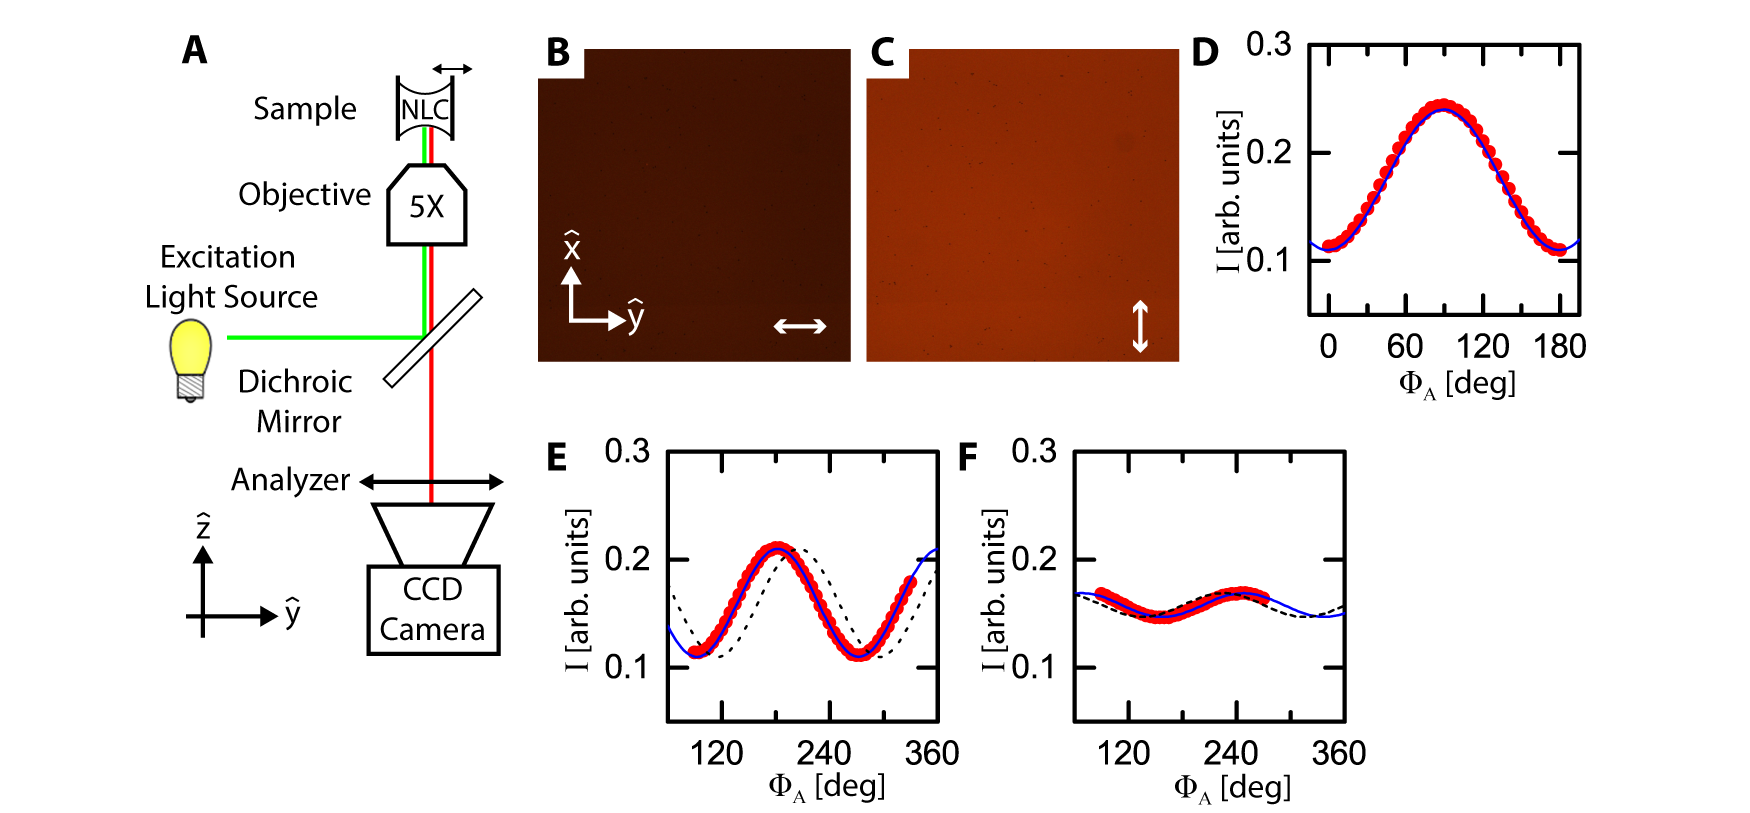
\includegraphics{figures/C5/Ch5-Figs_PFM_FlatCell.png}
  \caption{Polarized epifluorescent microscopy on a planar NLC cell filled with a mixture of 5CB and Nile Red.
  (A), Schematic from the side of the setup for polarized epifluorescent microscopy (PFM).
  (B--D), PFM (B,C) images and (D) recorded intensity as a function of $\Phi_A$ of the planar NLC cell with rubbing direction along $\hat{x}$.
  $\Phi_A$ is indicated in the images in (B,C), and is measured in (D) with respect to $\hat{y}$.
  The blue curve is a fit of the data to Eq.~\ref{e:5-IntFit}, returning $\delta' = 89^{\circ}$.
  (E,F), Recorded intensity as a function of $\Phi_A$ of the planar NLC cell with rubbing direction (E) 25$^{\circ}$ CCW from $\hat{y}$ and (F) 45$^{\circ}$ CCW from $\hat{y}$.
  The blue curves are fits of the data to Eq.~\ref{e:5-IntFit} and have $\delta' = 2^{\circ}$ and $\delta' = 67^{\circ}$, respectively.
  The black dashed lines correspond to theoretical curves for $\delta' = 25^{\circ}$ and $\delta' = 45^{\circ}$, respectively.}\label{f:5-PFM_FlatCell}
\end{figure}


\subsection{Experimental realization}
We add $0.01$ wt\% Nile red to 5CB; at this concentration, Nile red does not affect the director configuration~\cite{RN173}.
We image our sample using a standard epifluorescent setup with an analyzer in the emitted light path [Figure~\ref{f:5-PFM_FlatCell}(A)] and a short-arc lamp as our light source.
We use filter set \#20 from Zeiss, with a 534~nm~--~558~nm bandpass excitation filter, a 560~nm longpass dichroic mirror, and a 575~--~640~nm emission filter~\cite{RN288}.
For a sample, we record the output intensity $I(x,y)$ as a function of $\Phi_A$ and then fit the intensity at every pixel to the form:
\begin{equation}
    I(x,y) = A + B \cos^2{(\Phi_A-\delta'(x,y))},\label{e:5-IntFit}
\end{equation}
where $A$, $B$ and $\delta'$ are fitting parameters; $A$ and $B$ set the minimum value and range of $I$, respectively, and $\delta'$ reflects an average of the director orientation along the light path.
Using the extracted $\delta'$ values, we can then plot the associated director field for a sample.
\begin{figure}
  \centering
  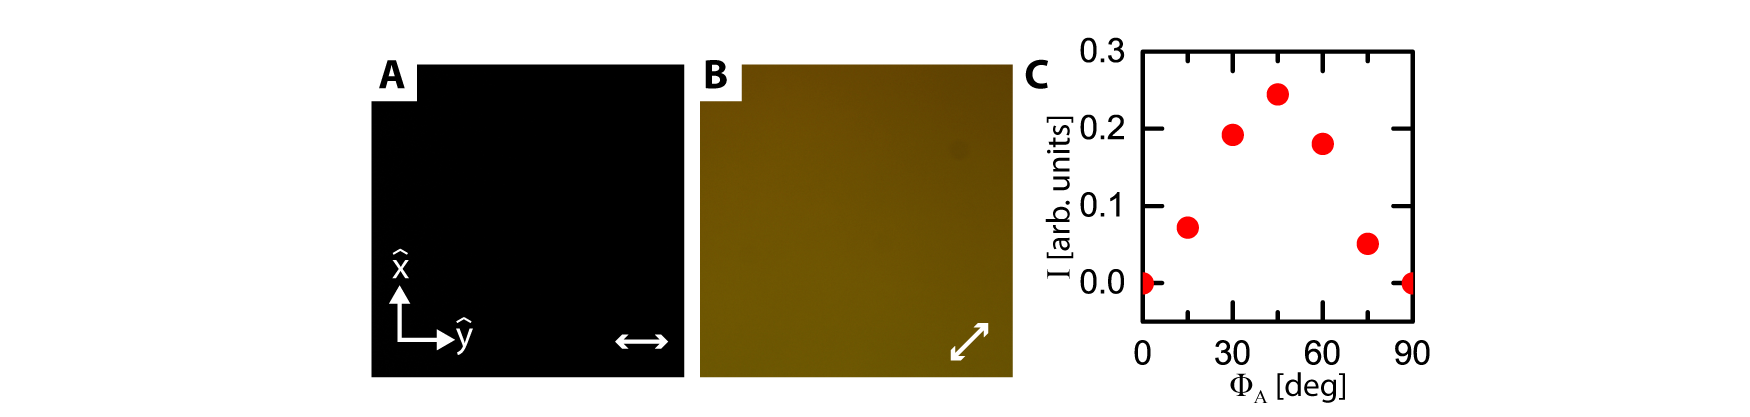
\includegraphics{figures/C5/Ch5-Figs_DichroicMirror.png}
  \caption{The dichroic mirror is birefringent.
  (A,B), Optical-polarized microscopy images with no sample, P and A crossed, and the dichroic mirror in the light path.
  $\Phi_A$ is indicated by the white arrow in the bottom-right of each image.
  (C), Transmitted intensity as a function of $\Phi_A$ for the same setup as in (A,B), with $\Phi_A$ measured CCW off of $\hat{y}$.
  The maximum at $\Phi_A = 45^{\circ}$ and minima at $\Phi_A = 0^{\circ},\, 90^{\circ}$ implies that the optic axis of the mirror is along either $\hat{x}$ or $\hat{y}$.}\label{f:5-DichroicMirror}
\end{figure}


We initially test our analysis on planar cells (INSTEC LC2-9.0) that we fill with 5CB via capillary action.
We image the cell with PFM and find that the fluorescence is much brighter when $\Phi_A$ is parallel to the rubbing direction than when $\Phi_A$ is perpendicular to the rubbing direction, as shown in Figure~\ref{f:5-PFM_FlatCell}(B,C), respectively, for a rubbing direction oriented along $\hat{x}$.
Plotting the average intensity in each image as a function of $\Phi_A$ with the (${\color{red} \bullet}$) symbols in Figure~\ref{f:5-PFM_FlatCell}(D), where $\Phi_A$ is measured off of $\hat{y}$, we see that the intensity varies as we would expect for such a rubbing direction: the intensity is a maximum when $\Phi_A = 90^{\circ}$ and a minimum when $\Phi_A = 0^{\circ}, \, 180^{\circ}$.
We fit the data in Figure~\ref{f:5-PFM_FlatCell}(D) to the expression in Eq.~\ref{e:5-IntFit} [blue curve] and find $\delta' = 89^{\circ}$, as expected.

We next change the rubbing direction to $25^{\circ}$ measured from $\hat{y}$ and plot the intensity as a function of $\Phi_A$ with the (${\color{red} \bullet}$) symbols in Figure~\ref{f:5-PFM_FlatCell}(E).
However, when we fit the data to Eq.~\ref{e:5-IntFit} [blue curve], we find $\delta' = 2^{\circ}$.
Plotting the theoretical curve for $\delta' =25^o$ [blue dashed line, Figure~\ref{f:5-PFM_FlatCell}(E)], we see that the data are shifted to the left of the expected values.
In addition, we see that the total intensity variation in the sample has decreased.
Similarly, when we do the same for a rubbing direction of $45^{\circ}$ [see Figure~\ref{f:5-PFM_FlatCell}(F)], the fit returns $\delta' = 67^{\circ}$, with the data now shifted to the right of the expected values [blue dashed line, Figure~\ref{f:5-PFM_FlatCell}(F)] and showing even less intensity variation.
We hypothesize that there is another birefringent element in the light path with its optic axis along $\hat{x}$ or $\hat{y}$; the additional retardation changes the linearly polarized light to elliptically polarized light, shifting the $I$ vs $\Phi_A$ curve and decreasing the variation in the light intensity as a function of $\Phi_A$.

We confirm this by taking OPM images with no sample and just the dichroic mirror still in the light path, as seen for P and A at $0^{\circ}$ and $90^{\circ}$ and at $45^{\circ}$ and $135^{\circ}$ in Figure~\ref{f:5-DichroicMirror}(A,B), respectively.
The bright image in Figure~\ref{f:5-DichroicMirror}(B) indicates the mirror is birefringent; plotting the transmitted intensity for crossed P and A as a function of $\Phi_A$ in Figure~\ref{f:5-DichroicMirror}(C), we see that the optic axis of the mirror is indeed along either $\hat{x}$ or $\hat{y}$.
While the mirror affects the quantitative results, we see from our experiments with the planar cell that we can still distinguish between different rubbing directions.
Finally, we also melt the 5CB in the cell to the isotropic to ensure that there is no appreciable intensity variation with changing $\Phi_A$, as shown by the relatively flat transmitted intensity curve in Figure~\ref{f:5-PFM_FlatCell}(J).
With the 5CB in the isotropic, we measure the range in the intensity variation as a function of $\Phi_A$ to be 6\% of the mean intensity.
We compare this to the cell with the rubbing direction along $45^{\circ}$, where our intensity variation with the 5CB in the nematic phase is the smallest, and find that the range in $I$ is 25\% of the mean.
This indicates that the intensity variation is due to the 5CB and not to some property of the cell.
\begin{figure}
  
\includegraphics{figures/C5/Ch5-Figs_IsotropicPlanar.png}
  \caption{Recorded intensity as a function of $\Phi_A$ of a planar NLC cell filled with 5CB and melted to the isotropic.
  The rubbing direction is along $90^o$ and the range in $I$ is 6\% of the mean.}\label{f:5-IsotropicPlanar}
\end{figure}


\subsection{Validation in spherical droplets and cylindrical capillaries}
We now turn to validating PFM using objects with a spatially varying director field.
We start by considering spherical droplets of the Nile red-doped 5CB in water, with 8 mM SDS in the water to enforce homeotropic anchoring, shown in the bright-field image in Figure~\ref{f:5-PFM_Spheres}(A).
We rotate the crossed P and A, as seen in Figure~\ref{f:5-PFM_Spheres}(B,C) for two different P and A orientations, and confirm that the droplets have the classic radial configuration~\cite{RN177}, with a single radial hedgehog at the center of each droplet.

Importantly, we also notice that when rotating the analyzer the entire image appears to translate along a circular trajectory.
Superimposing images of the spherical droplets with $\Phi_A = 0$ and $\Phi_A = \pi$ in Figure~\ref{f:5-PFM_Spheres}(D), we see that the images have been displaced.
This displacement comes from the analyzer; it has a wedge angle to prevent specular reflections from affecting the final image quality,.
However, this also serves to translate the image by $\Delta \rho$ along the orientation of the wedge angle, $\Phi_W$, as illustrated schematically in Figure~\ref{f:5-AnalyzerShift}(A).
Thus, rotating the analyzer by $\pi$ translates the image in a semicircle with radius $\Delta \rho$ [see Figure~\ref{f:5-AnalyzerShift}(B)].
This means that to properly consider $\delta'(x,y)$ as a function of $\Phi_A$, we have to correct this displacement so that $I(x,y)$ comes from the same $\delta'(x,y)$ for all $\Phi_A$.
\begin{figure}
  \centering
  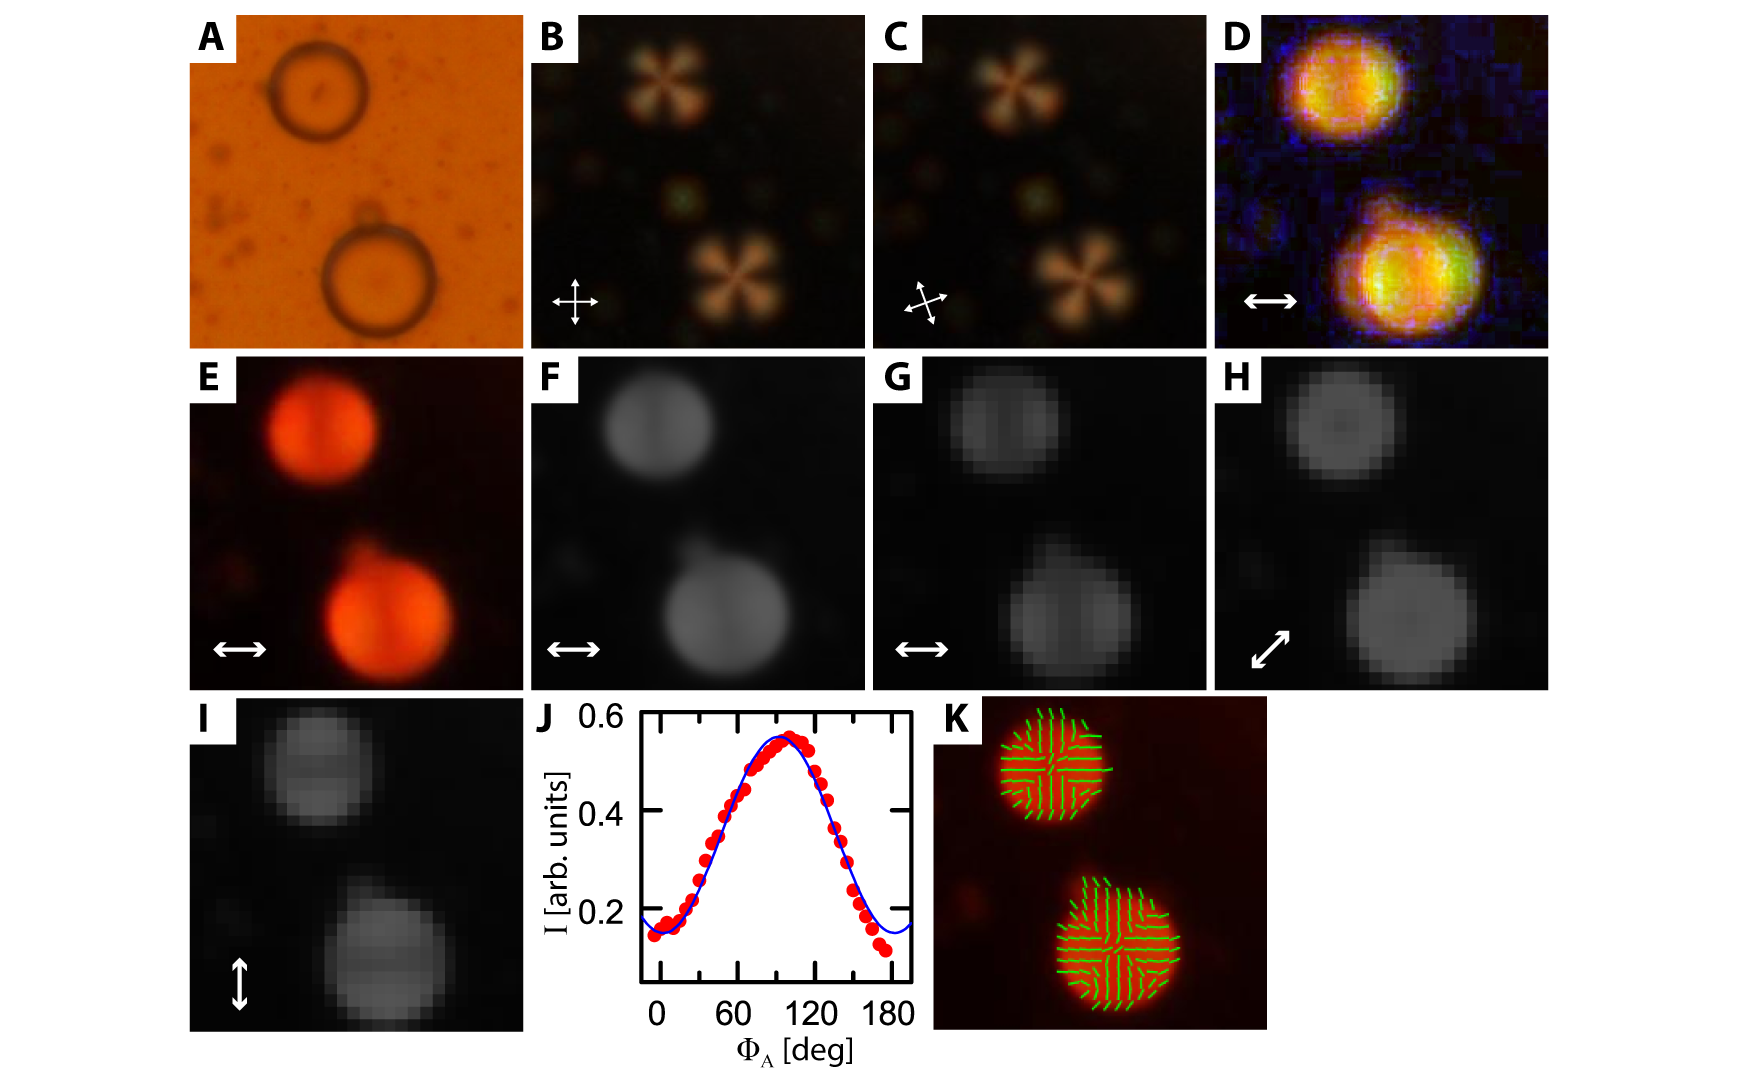
\includegraphics{figures/C5/Ch5-Figs_PFM_Spheres.png}
  \caption{PFM analysis for radial droplets.
  (A), Bright field image of radial droplets made from a mixture of 5CB and Nile red dispersed in water and 8 mM SDS.
  (B,C), Corresponding crossed-polar images of the droplets in (A) with the P and A orientation indicted in each image.
  The texture rotates with P and A, indicating the hedgehog in each droplet is radial.
  (D), Superposition of two PFM images of the droplets in (A), where the images have the same $\Phi_A$ but opposite analyzer wedge-angle orientations. Note how the two images are displaced due to the effect of the analyzer wedge-angle, making the superposition blurry.
  (E), Superposition of the same images in (D) after shifting each image to correct for the displacement due to the analyzer wedge-angle. Here, the two droplets are clear and the superposition is no longer blurry.
  The analyzer angle in (D,E) is indicated schematically.
  (F), Grayscale intensity of a PFM image of the droplets in (A) after blurring with a square Gaussian filter with side length 7 px.
  The analyzer orientation is indicated schematically.
  (G-I), Downsampled PFM images after blurring, with the analyzer angle in each image indicated schematically.
  (J), PFM intensity as a function of $\Phi_A$ from the highlighted pixel in (G-I).
  The blue curve is a fit to Eq~\ref{e:5-IntFit}, returning $\delta' = 88^{\circ}$.
  (K), The $\delta'$ from a PFM analysis of every pixel in (G-I) plotted on top of an epifluorescent image of the droplets.
  The droplets are clearly radial, matching our observations in (B,C).
  The scale bar in (A) is 25 $\upmu$m.}\label{f:5-PFM_Spheres}
\end{figure}

We accomplish this by translating all the images along their respective $\Phi_W$ by a fixed magnitude $\Delta \rho$, removing the effect of the displacement due to the analyzer wedge angle for each image.
Since $\Phi_W \in [0,\pi]$ while $\Phi_A \in [0, 2 \pi]$, we use $\Phi_A$ to determine $\Phi_W$ up to a factor of $\pi$ in each set of images; we translate an entire set by $\Delta \rho$ along both $\Phi_W = \Phi_A$ and along $\Phi_W = \Phi_A + \pi$ and keep the set where the displacement has been removed.
Note that in our microscope, $\Phi_A$ and $\Phi_W$ also differ by $30^{\circ}$ [see Figure~\ref{f:5-AnalyzerShift}(B)].
Our standard microscope setup with a $5\times$ objective and a $0.5 \times$ adapter in front of the camera (The Imaging Source, DFK 41BU02) has $\Delta \rho = 6$ px.

Now superimposing the corrected versions of the images used in Figure~\ref{f:5-PFM_Spheres}(D), we see in Figure~\ref{f:5-PFM_Spheres}(E) that the displacement between the two images has disappeared.
While in principle we could consider $\delta'(x,y)$ for every pixel, that is more information than we need and is susceptible to pixel-level noise.
Instead, we blur each image with a mean filter to both remove noise and locally average the $\delta'$, and then downsample each image to reduce the number of fits we need to perform.
We illustrate this with the example PFM images in Figure~\ref{f:5-PFM_Spheres}(F-I), where the analyzer angle is indicated in each image.
The original image is convolved with a mean filter of side length 7 px, yielding the blurred image in Figure~\ref{f:5-PFM_Spheres}(F) and then downsampled by a factor of 7, as displayed in Figure~\ref{f:5-PFM_Spheres}(G).
Here, we focus on the highlighted pixel in the downsampled images in Figure~\ref{f:5-PFM_Spheres}(G-I) and plot the intensity in Figure~\ref{f:5-PFM_Spheres}(J).
A fit of Eq~\ref{e:5-IntFit} to the data in Figure~\ref{f:5-PFM_Spheres}(J) yields $\delta' = 88^{\circ}$.
We do this for every pixel in the downsampled images and plot $\delta'(x,y)$ on top of the epifluorescent image in Figure~\ref{f:5-PFM_Spheres}(K).
Indeed, we see that we qualitatively capture the radial texture.
Note that we are unable to distinguish the actual point singularity due to the wide-field nature of our technique and the influence of the mirror; however, we clearly detect the presence of a radial defect in each droplet.
\begin{figure}
  \centering
  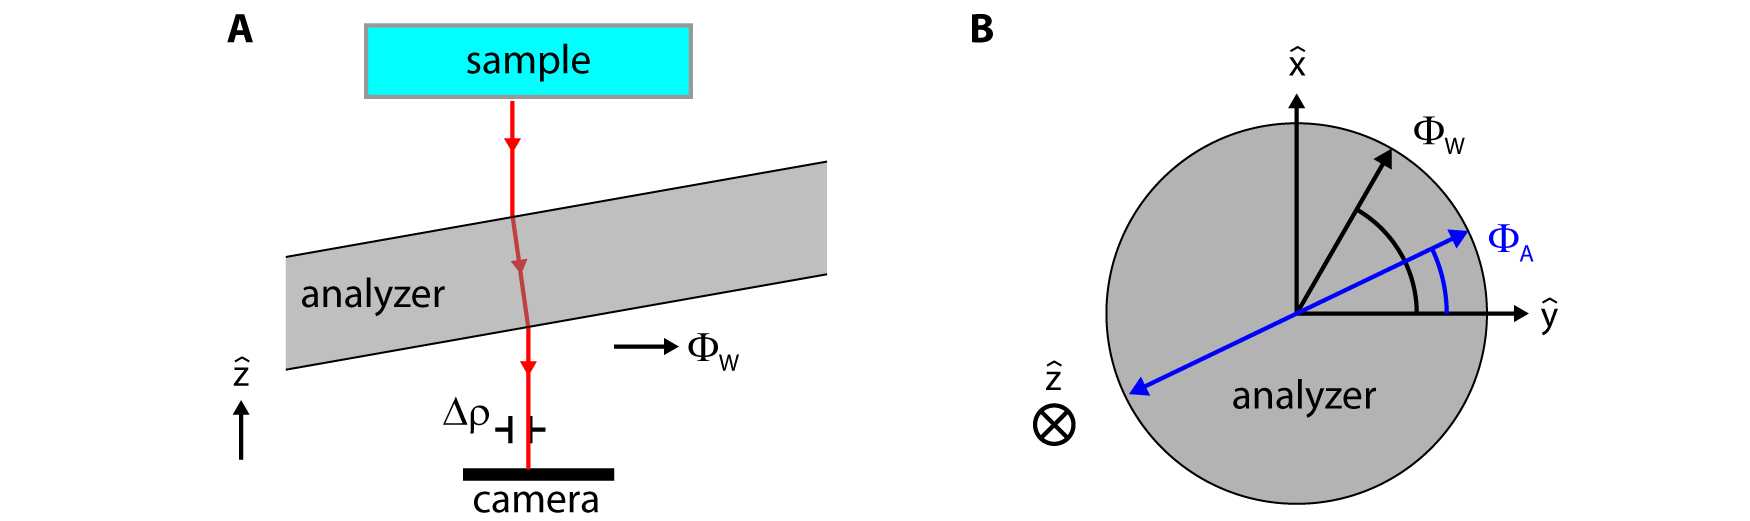
\includegraphics{figures/C5/Ch5-Figs_AnalyzerShift.png}
  \caption{The analyzer shifts the image.
  (A), Schematic from the side showing how the wedge angle of the analyzer causes light from the sample to be translated by $\Delta\rho$ in the direction of the wedge, $\Phi_W$.
  (B), The analyzer pass axis and the wedge angle are not parallel to each other.
  Rotating the analyzer by $\pi$ will translate the image on the camera along a semicircle with radius $\Delta\rho$.
  Since $\Phi_A \in [0, \pi]$ while $\Phi_W \in [0, 2 \pi]$, knowing $\Phi_A$ alone is not enough to know which direction the output image has been translated.}\label{f:5-AnalyzerShift}
\end{figure}

We next consider a cylindrical capillary filled with Nile red-doped 5CB.\@
The capillary has a 600 $\upmu$m inner diameter and is coated with lecithin to enforce homeotropic anchoring; it has a escaped-radial configuration with a point defect separating regions that escape in opposite directions~\cite{RN179}, as seen in the crossed-polar images in Figure~\ref{f:5-PFM_Capillary}(A).
We confirm that the defect is a radial point by rotating the crossed polarizer and analyzer and observing that the brushes follow the sense of rotation.
We then image the capillary using PFM, where we have shifted, blurred, and downsampled the images as with the radial droplets in Figure~\ref{f:5-PFM_Spheres}, and plot the output $\delta'$ on top of a bright-field image of the capillary in Figure~\ref{f:5-PFM_Capillary}(B).

As with the droplets, we see that we qualitatively capture the expected escaped-radial texture; we capture the radial character of the defect between the two escaped domains, but we do not resolve the singularity itself in our output.
Since the escaped-radial director field for 5CB has been analytically solved~\cite{RN289,RN290}, with $\mathbf{n}(r,\varphi,z) = \left \{ \sin(\Omega), 0, \cos(\Omega)   \right \}$, where $\Omega = 2 \arctan(r/R) $, with $R$ the capillary radius in cylindrical coordinates and $\hat{z}$ along the capillary axis, we can compare the theoretical $\Omega$ with our measured $\delta'$, as plotted in Figure~\ref{f:5-PFM_Capillary}(C).
% Again, we see deviation, with our results biased towards $0^{\circ}$ and $90^{\circ}$.
Even though there are quantitative differences, we can clearly see from both the plot of $\delta'$ vs $x/R$ [Figure~\ref{f:5-PFM_Capillary}(B)] and the plotted $\delta'$ fields [Figure~\ref{f:5-PFM_Capillary}(C)] that we capture the different escape directions and thus can also resolve the radial character of defect between them.
\begin{figure}
  \centering
  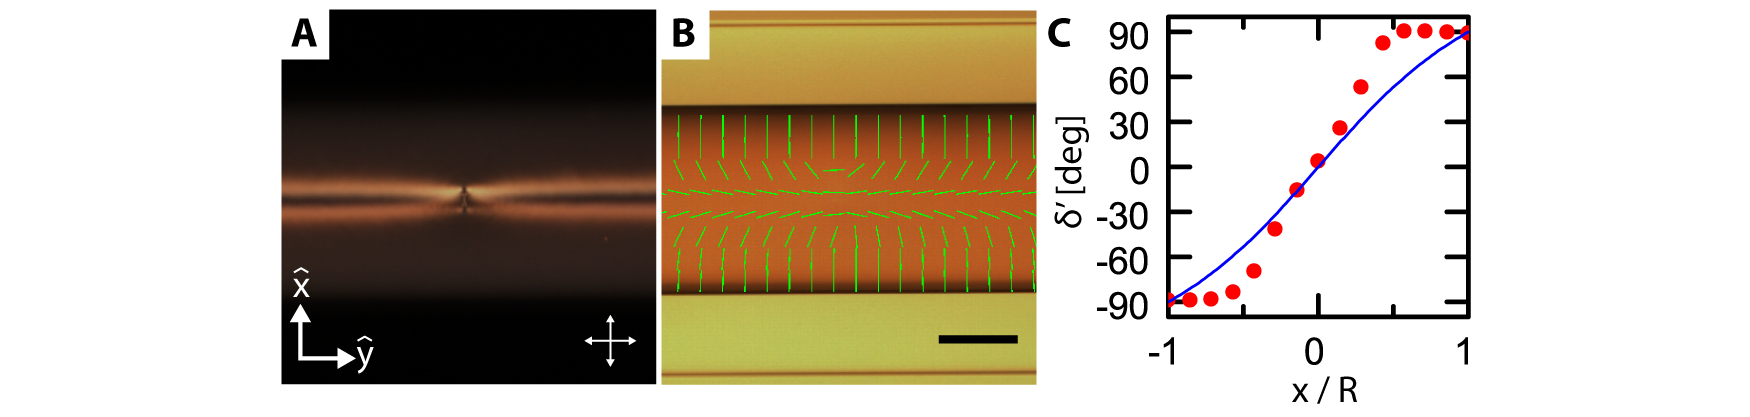
\includegraphics{figures/C5/Ch5-Figs_PFM_Capillary.png}
  \caption{PFM in an escaped-radial capillary.
  (A), Crossed-polar image of a capillary filled with the Nile Red-Doped 5CB under homeotropic anchoring.
  (B), Bright-field image of the capillary in (A), with the director orientation from the PFM analysis plotted on top of the associated bright-field image.
  (C), $\delta'$ plotted versus the position across the capillary for the column indicated by the red arrow in (B).
  The blue curve is $2 \arctan (x/R)$, the theoretical director angles for an escaped-radial configuration in the one-constant approximation.
  Using the 5CB value of $K_{11}/K_{33} = 0.74$ would only slightly change the blue curve.
  The scale bar in (B) is 250 $\upmu$m.}\label{f:5-PFM_Capillary}
\end{figure}

\subsection{Radial and hyperbolic defects in waists and barrels}
We now use PFM on our waist-shaped bridges to determine if the defect is radial or hyperbolic.
Since the output of PFM is biased due to the dichroic mirror, we orient the bridges with the plates along $45^{\circ}$, as seen in the bright-field image of a bridge in Figure~\ref{f:5-PFM_Bridge}(A), such that PFM will best distinguish the differences between a radial and a hyperbolic defect.
We start with the waist-shaped bridges; for each bridge we perform a PFM analysis and plot the $\delta'$ on top of an epifluorescent image, as shown for an example bridge with large $\Gamma$ in Figure~\ref{f:5-PFM_Bridge}(A,B) and an example bridge with small $\Gamma$ in Figure~\ref{f:5-PFM_Bridge}(C,D).
For both examples, we see that the defect structure is hyperbolic.
We do this for waist-shaped bridges spanning $\Gamma \ll \Gamma_c$ to $\Gamma \gg \Gamma_c$, and find that the defect is always hyperbolic, implying that our waist-shaped bridges undergo transitions from a hyperbolic ring to a hyperbolic point as $\Gamma$ decreases.
\begin{figure}
  \centering
  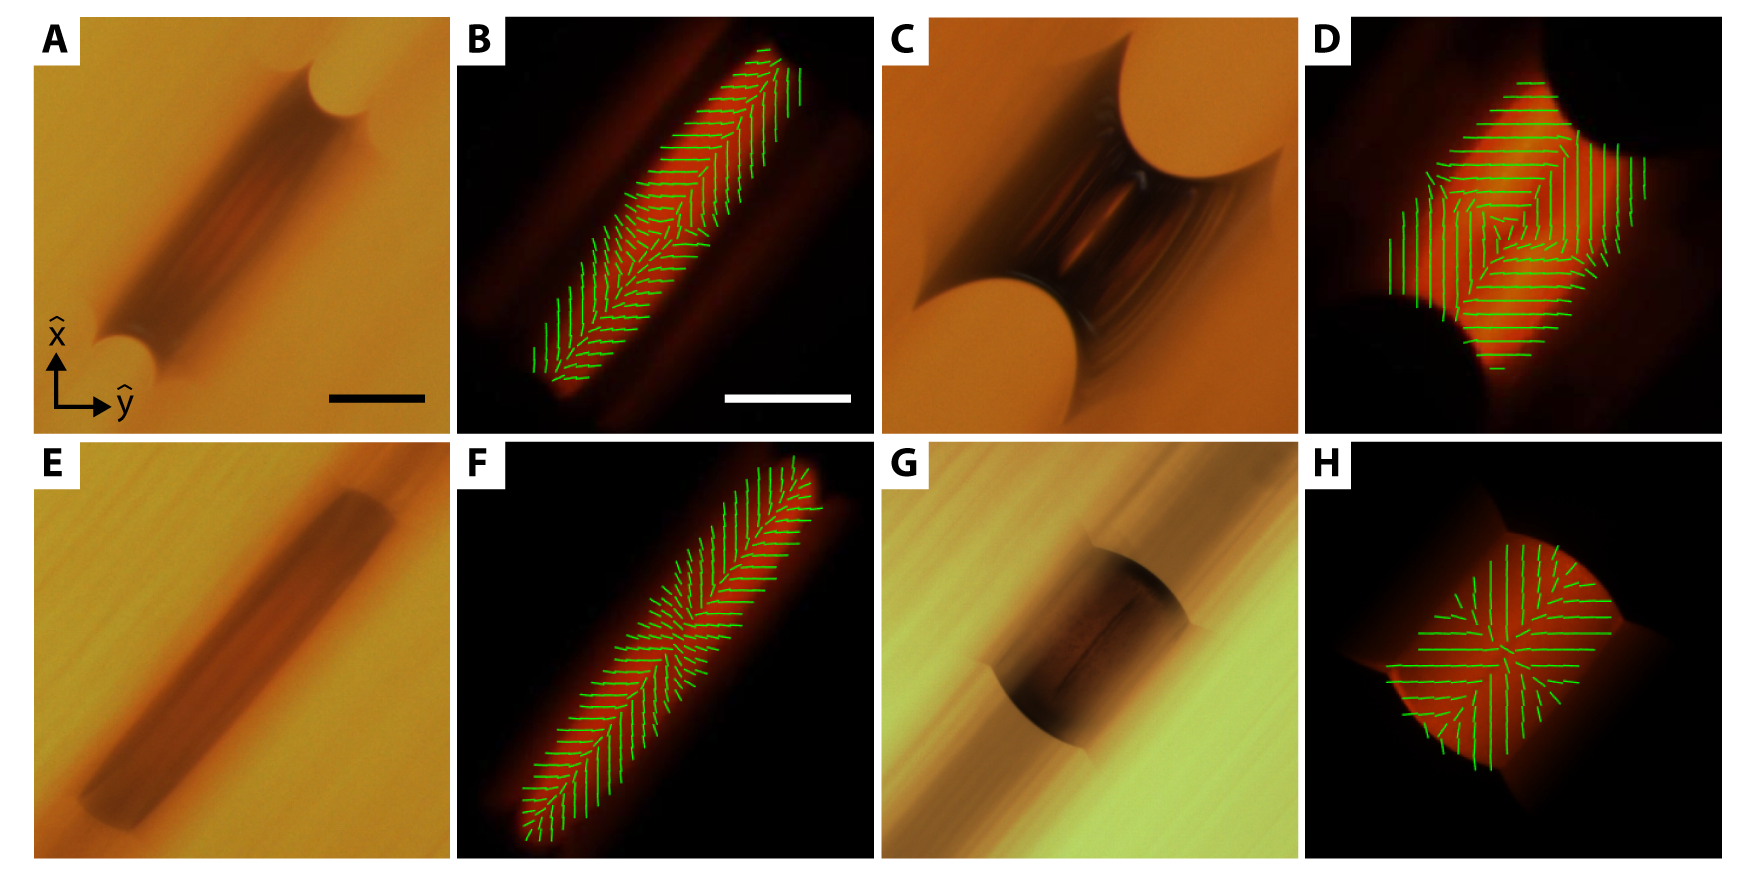
\includegraphics{figures/C5/Ch5-Figs_PFM_Bridge.png}
  \caption{(A-D), PFM analysis on waist-shaped bridges with (A,B) $\Gamma = 4.0$ and (C,D) $\Gamma = 0.8$.
  The $\delta'$ are plotted on the epifluorescent images in (B,D) with the associated bright-field images in (A,C).
  (E-H), PFM analysis on barrel-shaped bridges with (E,F) $\Gamma = 6.6$ and (G,H) $\Gamma = 1.5$.
 The $\delta'$ are plotted on the epifluorescent images in (F,H) with the associated bright-field images in (E,G).
 The scale bars in (A,B) are 250 $\upmu$m, with the scale for all the (A,C,E,G) bright field images and all the (B,D,F,H) PFM images the same.}\label{f:5-PFM_Bridge}
\end{figure}

We now turn to barrel-shaped bridges, where we add the water and SDS mixture when the 5CB is in the isotropic phase, and we consider barrels made with both a large and a small initial $\Gamma$.
As demonstrated in the plots of $\delta'$ on top of epifluorescent images of two example barrels with different $\Gamma$ in Figure~\ref{f:5-PFM_Bridge}(E-H), the barrel-shaped bridges at all measured $\Gamma$ have radial defects.
Thus, we see that the shape of the bridge, driven by the contact angle, determines if the defect is radial or hyperbolic.
This makes sense intuitively as the homeotropic boundary conditions cause the boundary to act as a level surface for the director.

Due to the ability of shape to bias the defect structure, the cylindrical bridge becomes an interestingly peculiar case, as the shape is neither a waist nor a barrel.
While accomplishing this experimentally in our system would be technically difficult due to the requirement of maintaining $\Theta_0 = 90^{\circ}$, we can turn to numerical calculations to explore this scenario.




\section{Comparison with numerical calculations: stable and metastable states}
We compare our results with numerical calculations performed by Shengnan Huang and Paul Goldbart.
These assume the problem is completely 2D; for a bridge parameterized in cylindrical coordinates, $\mathbf{n}(r,\varphi,z) = \left \{ \sin(\Omega), 0, \cos(\Omega)   \right \}$, where $\Omega = f(r,z)$ only.
We then minimize the free-energy using a version of the finite difference method laid out in Ref.~\cite{RN144}, modified as follows.
Although the free energy in the algorithm presented there depends on the cut-off length of the defect core, the equilibrium defect configuration is independent of this length scale provided it is reasonably small.
We modify the algorithm to treat the small region containing the defect separately from the remainder of the computation volume, such that the calculated free energy converges as the mesh size grows~\cite{RN199,RN200,RN201}.

A cylindrical bridge is considered first.
For the 5CB values of $K_{11}/K_{33} = 0.74$, a bridge should undergo a defect transition between a radial ring and a hyperbolic point, as highlighted by the dashed line in the phase diagram in Figure~\ref{f:5-Calcs}(A).
This result is consistent with prior computational modeling~\cite{RN144}, and highlights the peculiarity of the cylindrical case.
However, the calculations find ring-to-point defect transitions at aspect ratios that are significantly smaller than previously reported~\cite{RN144}.
In addition, in contrast to prior modeling, the calculations show no transition to a radial point structure~\cite{RN144}; only the hyperbolic point structure is stable [Figure~\ref{f:5-Calcs}(A)].
Instead, the numerical calculations predict that the radius of the radial ring should vary linearly with $\Gamma$ for the entire range of $\Gamma$ explored.
\begin{figure}
  \centering
  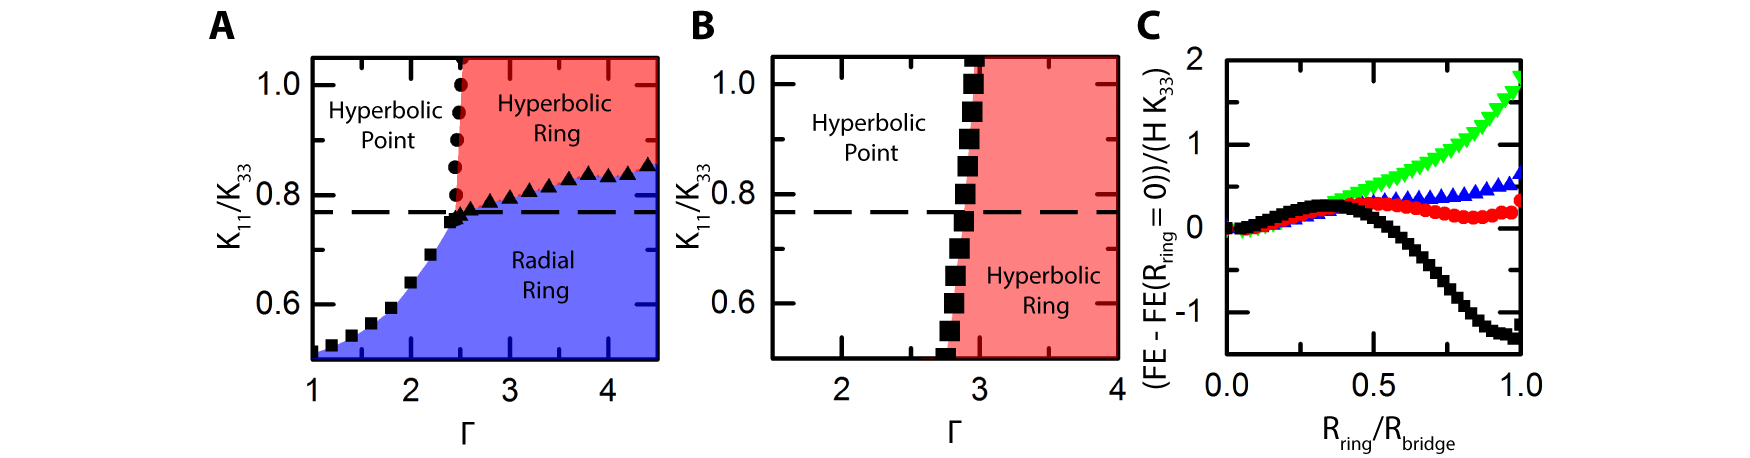
\includegraphics{figures/C5/Ch5-Figs_Calcs.png}
  \caption{Results from the computational modeling of a nematic in a capillary bridge.
  (A), Phase diagram of the defect structure in a cylinder as a function of aspect ratio $\Gamma$ and the ratio, $K_{11}/K_{33}$, of the splay and bend elastic constants.
  (B), Phase diagram of the defect structure in a waist-shaped bridge as a function of $\Gamma$ and $K_{11}/K_{33}$.
  In (A,B), the minimum-energy state is indicated in each region, and the dashed line corresponds to $K_{11} / K_{33}$ for 5CB.\@
  (C,D), Free energy of a director configuration in a waist-shaped bridge relative to the free energy in the presence of the point defect and normalized by $H K_{33}$, shown as a function of scaled ring radius $R_{ring}/R_{bridge}$.
  The curves correspond to (${\blacksquare}$) $\Gamma = 3.5$, (${\color{red} \bullet}$) $\Gamma = 2.8$, (${\color{blue} \blacktriangle}$) $\Gamma = 2.5$, and (${\color{green} \blacktriangledown}$) $\Gamma = 2.0$.}\label{f:5-Calcs}
\end{figure}

Next, the shape of the boundaries in the numerical calculations are changed.
Consistent with our experiments, it is found that the radial defects in the phase diagram for a waist-shaped bridge disappear for all values of $K_{11}/K_{33}$ used, as shown in Figure~\ref{f:5-Calcs}(B).
Furthermore, the ring defect radius in Figure~\ref{f:5-ExpWaistTop}(F) predicted by the calculations (${\color{red} \bullet}$) for a waist-like shape agrees very well with our experimental data ($\blacksquare$).
In addition, the hyperbolic-ring to hyperbolic-point transition is found to happen at $\Gamma_c = 2.7$ for $K_{11}/K_{33} = 0.74$ [dashed line, Figure~\ref{f:5-Calcs}(B)], in agreement with our experimental measurement of $\Gamma_c = 2.7 \pm 0.3$ for decreasing $\Gamma$.

To investigate the hysteresis in our experimental hyperbolic ring to hyperbolic point transition, the energy landscape of a waist-shaped nematic bridge as a function of ring radius is calculated.
Results for two bridges having $\Gamma > \Gamma_c$ and for two bridges having $\Gamma < \Gamma_c$ are shown in Figure~\ref{f:5-Calcs}(C,D), where we have taken $K_{11}/K_{33} = 0.74$; recall that the point defect is represented by the free energy for a vanishing ring radius.
As the free energy exhibits a local minimum at $R_{ring} = 0$ [Figure~\ref{f:5-Calcs}(D)], we indeed see that the point defect is metastable for $\Gamma > \Gamma_c$, consistent with our interpretation of the experimental results.
In addition, given a representative bridge height of $H = 100$ $\upmu$m and $K_{33} \approx 10^{-11}$ N, we find that the height of the barrier is always $\mathcal{O} \left ( 10^{4} \right )$ k$_\textrm{B}$T, implying that a point defect will not spontaneously transform into a ring defect over the duration of our experiments, also consistent with our experimental observations.
For $\Gamma < \Gamma_c$, this metastability disappears, and the hyperbolic point defect is the only stable defect state.

Turning to barrel-shaped bridges, the calculations show that all hyperbolic defects disappear from the phase diagram, leaving the radial ring as the only equilibrium state for the range of $\Gamma$ and $K_{11/K_{33}}$ explored.
This confirms that the shape of the free surface determines if the enclosed defect is radial or hyperbolic.
Barrel-like shapes with positive Gaussian curvature favor radial defects and waist-like shapes with negative Gaussian curvature favor hyperbolic defects.
We also see that the ring radius in Figure~\ref{f:5-ExpBarrelRing}(A) predicted by the calculations (${\color{olive} \bullet}$) in a barrel-shaped bridge also agrees with our experimental results (squares), despite the influence of the SDS micelles in the experiments.




\section{Conclusions}
In conclusion, the equilibrium defect structure in a nematic capillary bridge under homeotropic boundary conditions is found to depend on both the shape of the bounding surface as well as the aspect ratio of the bridge.
The aspect ratio determines whether the defect is a ring defect or a point defect, and the boundary shape determines whether the defect is radial or hyperbolic, with waist-like shapes containing hyperbolic defects and barrel-like shapes containing radial defects.
In addition, we find that in a waist structure the point defect can be metastable,  causing the transition between a ring defect and a point defect to exhibit hysteresis.
Starting at $\Gamma > \Gamma_c$ and decreasing $\Gamma$ to below $\Gamma_c$ brings about the collapse of the ring defect to a point defect, with the collapse occurring at a nonzero value of the ring radius.
However, starting with a point defect at $\Gamma < \Gamma_c$ and increasing $\Gamma$ never yields a transition from a point defect to a ring defect.

Although prior computations with thin films~\cite{RN141} or perforated sheets~\cite{RN149} have been used to attribute the radial or hyperbolic character of defects to confinement shape, our work provides the first experimental evidence of this phenomenon.
We accomplish this by developing PFM, a simpler technique than its confocal counterpart that enables us, despite the influence of refraction from the surface of the bridge, to determine the director field when viewing the bridge from the side.
Thus, our work confirms that curved geometries can be used to influence and control the equilibrium defect states in confined NLC under homeotropic boundary conditions.

As mentioned earlier, the cylindrical bridge with the predicted hyperbolic ring to radial point transition is a peculiar case.
Specifically, we note that a hyperbolic ring can become a hyperbolic point and a radial ring can become a radial point simply by shrinking $R_{ring}$ until $R_{ring} = 0$.
However, the predicted transition between a radial ring and a hyperbolic point [see Figure~\ref{f:5-Calcs}(A)] requires the director field to reorient throughout the entire bridge at some point during the transition.
The specific pathway for this transition is unclear and would be an interesting direction for future work.
Similarly, the phase diagram [Figure~\ref{f:5-Calcs}(A)] also predicts an equally intriguing transition between a radial ring and a hyperbolic ring.
Further interesting results would also be expected if the shape of the bridge is not fixed by surface tension, but can instead change and contribute to the free energy minimization \cite{RN12}.
Our work is thus one of many interesting studies that can be performed with nematic bridges to probe how shape and elasticity dictate the equilibrium defect structure of the liquid crystal.
